\documentclass[10pt]{article}
\usepackage[a4paper,margin=0.9in]{geometry}
\usepackage{booktabs,graphicx,amsmath,hyperref,caption,longtable,float,array,xcolor,microtype,enumitem,pdflscape,url}
\usepackage{placeins}
\usepackage[T1]{fontenc}
\hypersetup{colorlinks=true,linkcolor=blue!50!black,urlcolor=blue!50!black,citecolor=blue!50!black,
  pdftitle={Memory-lean density-fitted GPU4PySCF on P100, V100 and A100 GPUs},pdfauthor={Qing Shao}}
\captionsetup{font=small,labelfont=bf}
\setlength{\parskip}{3pt}
\renewcommand{\topfraction}{0.9}\renewcommand{\bottomfraction}{0.8}\renewcommand{\textfraction}{0.1}\renewcommand{\floatpagefraction}{0.7}\setcounter{topnumber}{3}\setcounter{totalnumber}{5}
\emergencystretch=2em
\graphicspath{{figures/}}
\newcommand{\BiggestAOs}{3336}
\newcommand{\BiggestAtoms}{417}
\newcommand{\BiggestName}{(H$_2$O)$_{139}$}
\newcommand{\CPULaneNote}{}
\newcommand{\CPUMaxBestAHund}{328}
\newcommand{\CPUMaxBestPSixteen}{197}
\newcommand{\CPUMaxBestVHund}{331}
\newcommand{\CPUMaxWideAHund}{2403}
\newcommand{\CPUMaxWidePSixteen}{1428}
\newcommand{\CPUMaxWideVHund}{2367}
\newcommand{\CPUMedBestAHund}{46}
\newcommand{\CPUMedBestPSixteen}{23}
\newcommand{\CPUMedBestVHund}{36}
\newcommand{\CPUMedWideAHund}{55}
\newcommand{\CPUMedWidePSixteen}{33}
\newcommand{\CPUMedWideVHund}{45}
\newcommand{\CPUNBestAHund}{41}
\newcommand{\CPUNBestPSixteen}{38}
\newcommand{\CPUNBestVHund}{41}
\newcommand{\CPUNWideAHund}{41}
\newcommand{\CPUNWidePSixteen}{38}
\newcommand{\CPUNWideVHund}{41}
\newcommand{\MaxAllAHund}{1.04}
\newcommand{\MaxAllAHundCupy}{2.39}
\newcommand{\MaxAllPSixteen}{1.63}
\newcommand{\MaxAllPTwelve}{2.26}
\newcommand{\MaxAllVHund}{1.09}
\newcommand{\MaxAllVHundCupy}{1.76}
\newcommand{\MaxBigAHund}{1.03}
\newcommand{\MaxBigAHundCupy}{2.39}
\newcommand{\MaxBigPSixteen}{1.63}
\newcommand{\MaxBigPTwelve}{2.26}
\newcommand{\MaxBigVHund}{1.09}
\newcommand{\MaxBigVHundCupy}{1.76}
\newcommand{\MedianAllAHund}{1.00}
\newcommand{\MedianAllAHundCupy}{1.01}
\newcommand{\MedianAllPSixteen}{1.01}
\newcommand{\MedianAllPTwelve}{1.02}
\newcommand{\MedianAllVHund}{1.00}
\newcommand{\MedianAllVHundCupy}{1.01}
\newcommand{\MedianBigAHund}{1.00}
\newcommand{\MedianBigAHundCupy}{1.02}
\newcommand{\MedianBigPSixteen}{1.04}
\newcommand{\MedianBigPTwelve}{1.05}
\newcommand{\MedianBigVHund}{1.00}
\newcommand{\MedianBigVHundCupy}{1.03}
\newcommand{\MemMax}{4.8}
\newcommand{\MemMedian}{2.1}
\newcommand{\MemMin}{1.00}
\newcommand{\MemN}{55}
\newcommand{\MinAllAHund}{0.88}
\newcommand{\MinAllAHundCupy}{0.95}
\newcommand{\MinAllPSixteen}{0.97}
\newcommand{\MinAllPTwelve}{0.90}
\newcommand{\MinAllVHund}{0.91}
\newcommand{\MinAllVHundCupy}{0.91}
\newcommand{\MinBigAHund}{0.91}
\newcommand{\MinBigAHundCupy}{0.99}
\newcommand{\MinBigPSixteen}{1.00}
\newcommand{\MinBigPTwelve}{0.99}
\newcommand{\MinBigVHund}{0.94}
\newcommand{\MinBigVHundCupy}{0.91}
\newcommand{\NAllAHund}{110}
\newcommand{\NAllAHundCupy}{109}
\newcommand{\NAllPSixteen}{104}
\newcommand{\NAllPTwelve}{107}
\newcommand{\NAllVHund}{110}
\newcommand{\NAllVHundCupy}{110}
\newcommand{\NAuditedRecords}{14\,648}
\newcommand{\NBigAHund}{32}
\newcommand{\NBigAHundCupy}{35}
\newcommand{\NBigPSixteen}{32}
\newcommand{\NBigPTwelve}{36}
\newcommand{\NBigVHund}{31}
\newcommand{\NBigVHundCupy}{33}
\newcommand{\NCasesRun}{127}
\newcommand{\NRecAHund}{2384}
\newcommand{\NRecAHundCupy}{2247}
\newcommand{\NRecPSixteen}{2184}
\newcommand{\NRecPTwelve}{2193}
\newcommand{\NRecVHund}{2399}
\newcommand{\NRecVHundCupy}{2265}
\newcommand{\NStrata}{7}

\newcommand{\gnew}{\textsc{new}}
\newcommand{\gold}{\textsc{orig}}

\title{Memory-lean density-fitted GPU4PySCF on P100, V100 and A100 GPUs:\\ accuracy, speed and capacity against the original code and CPU PySCF}
\author{Qing Shao\\\small Department of Chemical and Materials Engineering, University of Kentucky\\\small \texttt{qshao@uky.edu}}
\date{October 2026}

\begin{document}
\maketitle

\begin{abstract}
\noindent We benchmark a set of changes to the density-fitted single-GPU path of GPU4PySCF (a bounded fitted-integral build, a new disk tier next to the existing host-memory tier, cuBLAS contraction fast paths, and a lower-memory analytic gradient) against the unmodified upstream code and against CPU PySCF 2.14.0. The campaign covers \NCasesRun{} cases (SCF energies and gradients from H$_2$O to Taxol with six methods, Hessians, TDA and TDDFT, DF-MP2, CCSD, polarizabilities, shielding, solvation, dispersion, effective-core potentials, geometry optimizations and periodic systems) on P100 (12 and 16\,GB), V100 (16 and 32\,GB) and A100 (80\,GB) GPUs, with two contraction engines (cuTENSOR and the CuPy fallback) and three storage tiers, in \NAuditedRecords{} audited records with accuracy recomputed against an independent CPU result.

\noindent\textbf{Accuracy.} Wherever a result qualified, original and new code agree with the CPU to within the declared gates (worst energy error $8.6\times10^{-9}$~Eh against $10^{-8}$; worst gradient $9.0\times10^{-7}$~Eh/Bohr for the original and $8.5\times10^{-8}$~Eh/Bohr for the new code against $10^{-6}$). The original code fails the gradient gate on Taxol with hybrid functionals; wB97M-V and periodic MgO fail for both versions identically.

\noindent\textbf{Speed.} With cuTENSOR (V100, A100) the new code is as fast as the original (median original/new time ratio \MedianAllAHund{} on the A100 and \MedianAllVHund{} on the V100; per-case ranges \MinAllAHund--\MaxAllAHund{} and \MinAllVHund--\MaxAllVHund), with slowdowns of up to 12\% in individual Hartree--Fock and hybrid-functional cases. Without cuTENSOR (the P100 cards and a forced CuPy engine on V100 and A100) it is faster: 1.2--1.8$\times$ for intermediate-size hybrid-functional jobs and up to \MaxAllAHundCupy$\times$, where the original code pays for \texttt{einsum}. Job types that do not call the modified Fock-build and gradient paths directly (TDDFT, MP2, CCSD, properties, periodic) show no difference, and Hessians and optimizations differ by a few percent at most.

\noindent\textbf{Memory and capacity.} On the V100 the new code uses a median of \MemMedian$\times$ (up to \MemMax$\times$) less tracked GPU memory over the \MemN{} cases whose original peak exceeds 0.3\,GB (medians of 1.8--2.5$\times$ and maxima of 4.0--8.6$\times$ across the six strata). Combined with the host and disk tiers it lets a 12\,GB P100 run valinomycin (1542 basis functions) and an 80\,GB A100 a cluster of 139 water molecules (\BiggestAtoms{} atoms, \BiggestAOs{} basis functions), against a 537-function limit for the original code on the P100 cards (CuPy engine) and 2400 functions on the A100. Larger systems are limited by a gradient tensor of $N_\mathrm{aux}N_\mathrm{occ}^2$ elements, not by the fitted integrals.

\noindent\textbf{Comparison with the CPU.} The GPU is a median of \CPUMedBestAHund$\times$ (A100) and \CPUMedBestVHund$\times$ (V100) faster than the best available CPU lane for cases that take the CPU at least 20\,s, and up to \CPUMaxBestAHund$\times$ (A100) for finite-difference Hessians; a whole-node 48-thread CPU run was found to be slower than a 24-thread, single-BLAS-thread run in 120 of the 123 cases with both lanes (median 2.0$\times$ for the 65 cases above 20\,s on 48 threads, up to 33$\times$ for a Hessian) because of nested BLAS threading, and both are reported.
\end{abstract}


\noindent\textbf{Keywords:} GPU computing, density functional theory, density fitting, PySCF, GPU4PySCF, benchmarking, quantum chemistry

\section{Introduction}

Graphics processing units (GPUs) have become a routine target for electronic-structure software. GPU4PySCF~\cite{li2024gpu4pyscf,wu2024gpu4pyscf} accelerates the density-functional and related methods of PySCF~\cite{sun2018pyscf,sun2020pyscf} on NVIDIA GPUs, and its density-fitted (DF) single-GPU path~\cite{whitten1973,dunlap1979,vahtras1993} is the workhorse for medium-size molecules. Three practical limits recur when such code runs on the heterogeneous GPUs found in university clusters: the \emph{memory} of the card (12--16\,GB on older cards, 80\,GB on the largest), the \emph{contraction engine} available (cuTENSOR may be missing or unsupported, in which case NumPy-style \texttt{einsum} contractions in CuPy~\cite{okuta2017cupy} are used instead), and the need to know that a faster or smaller code gives \emph{the same answer}.

This paper evaluates a set of changes to the DF single-GPU path of GPU4PySCF: a bounded fitted-integral build workspace with a disk tier alongside the existing host-memory tier, cuBLAS contraction fast paths for the Fock build, and a lower-memory analytic gradient. We compare it with the unmodified upstream code and with CPU PySCF on three GPU generations. We ask two questions:

\begin{enumerate}[itemsep=1pt]
\item Does the new code give \emph{the same answer} as the original and as CPU PySCF across many job types, and is it \emph{faster}?
\item Does it let \emph{smaller-memory} GPUs treat \emph{larger systems}, and what does this cost in time?
\end{enumerate}

The measurements cover 127 benchmark cases on a university HPC cluster (the Lipscomb Compute Cluster, LCC) with P100 (12 and 16\,GB), V100 (16 and 32\,GB) and A100 (80\,GB) cards, two contraction engines (cuTENSOR and the CuPy fallback) and three storage tiers for the fitted integrals. The CPU serves as an accuracy oracle and, in a separate lane, as a timing baseline; the emphasis is on the GPU code, and the CPU baseline is required only to be fair. The accuracy criteria were declared before any performance run, and an independent audit recomputes every statistic from the stored records.

The main results are as follows. The new code is numerically equivalent to the original within the declared gates. With cuTENSOR it is not faster than the original; without cuTENSOR it is up to 2.4 times faster. Its main benefit is memory: a median of about 2 times less tracked GPU memory (up to 4.8 times on the V100 and 8.6 times on the A100), which lets a 12\,GB card treat a system of 1542 basis functions and an 80\,GB card one of 3336. We also report a caveat for CPU baselines: a whole-node 48-thread run with default BLAS threading is usually slower than a 24-thread run with one BLAS thread, so GPU-over-CPU speed-ups depend strongly on how the baseline is run.

Section~\ref{sec:methods} describes the code versions, hardware, cases, accuracy gates and timing protocol, including every deviation from the original plan. Section~\ref{sec:audit} describes the audit. Sections~\ref{sec:accuracy}--\ref{sec:cpu} give accuracy, speed, profiling and CPU-baseline results, and Section~\ref{sec:memory} the memory and capacity results. Section~\ref{sec:discussion} discusses when the new code helps and what limits larger systems, Section~\ref{sec:limits} the limitations, and Section~\ref{sec:conclusions} the conclusions.

\section{Experimental design}
\label{sec:methods}

\subsection{Code versions and the three-way comparison}

Three implementations are compared on identical inputs. G0 is called the original code and G1 the new code below. G0 is called the original code and G1 the new code below.

\begin{description}[leftmargin=1.2cm,style=nextline]
\item[\textbf{CPU}] PySCF~2.14.0~\cite{sun2018pyscf,sun2020pyscf} with density fitting, the matching physical model for every case. It serves as the accuracy oracle and, in a separate lane, as the CPU timing baseline.
\item[\textbf{G0 (original GPU)}] GPU4PySCF at upstream commit \texttt{9af748a}, with its Python sources unchanged.
\item[\textbf{G1 (new GPU)}] The reviewed working tree of the \texttt{improve-single-gpu} branch at the time the campaign was frozen. Relative to G0 it changes the density-fitted (DF) fitted-integral storage (a bounded build workspace and a new disk tier; the host-memory tier already exists upstream), the Coulomb and exchange contractions used by the DF Fock build (cuBLAS GEMM, GEMV and SYRK fast paths that bypass \texttt{einsum} when the CuPy contraction engine is active), the DF analytic gradient (bounded temporary workspace, in-place application of the auxiliary metric, a copy-free auxiliary Gram matrix for the CuPy engine, explicit cuBLAS stream binding), a density-evaluation shortcut in the GGA XC quadrature, and the CMake architecture selection. Several further changes were made while preparing the campaign, all verified before the freeze (Section~\ref{sec:deviations}).
\end{description}

G0 and G1 share one native library stack, built once for compute capabilities 6.0, 7.0, 8.0 and 9.0 (9.0 for completeness; no card of this study uses it) (9.0 for completeness; no card of this study uses it) with CUDA~12.4 and LibXC~7.1.2~\cite{lehtola2018libxc} compiled from source, so a single build serves every card. No native numerical kernel differs between G0 and G1; the comparison therefore isolates the Python-level algorithms and memory management. The contraction engine is an environment property and is recorded in every record: \textbf{cuTENSOR} (CuPy~13.4.1~\cite{okuta2017cupy} with cuTENSOR~2.2.0~\cite{cutensor}, used wherever installed) or the \textbf{CuPy fallback} (\texttt{CONTRACT\_ENGINE=cupy}, \texttt{einsum}-based). The fallback is the situation on hardware without a usable cuTENSOR, and it was the situation of an earlier single-GPU study of this branch on an NVIDIA GB10; here it is run deliberately on the V100 and A100 and is the only engine used on the P100 cards.

\subsection{Hardware strata}

Every card is a separate stratum and results are never pooled across strata. The V100-16 card was used only in the capacity study, so the audited campaign has six GPU stratum--engine combinations (A100, V100, P100-16 and P100-12 with their default engines, and A100 and V100 with the CuPy engine). Every GPU job uses one GPU and eight CPU cores (16 for the capacity study, which also takes the whole node memory).

\begin{table}[!htbp]
\centering\small
\resizebox{\textwidth}{!}{%
\begin{tabular}{llllll}
\toprule
stratum & GPU & compute cap. & memory & host & engine \\
\midrule
A100 & A100 PCIe 80\,GB & 8.0 & 80\,GB & Ice Lake, 56 cores, 256\,GB & cuTENSOR, CuPy \\
V100 & V100-SXM2 32\,GB & 7.0 & 32\,GB & Skylake, 32 cores, 192\,GB & cuTENSOR, CuPy \\
V100-16 & V100-SXM2 16\,GB & 7.0 & 16\,GB & Skylake, 32 cores, 192\,GB & cuTENSOR (capacity only) \\
P100-16 & P100-SXM2 16\,GB & 6.0 & 16\,GB & Haswell, 16 cores, 128\,GB & CuPy \\
P100-12 & P100-PCIe 12\,GB & 6.0 & 12\,GB & Skylake, 32 cores, 192\,GB & CuPy \\
CPU & -- & -- & -- & Cascade Lake, 48 cores, 192\,GB & -- \\
\bottomrule
\end{tabular}}
\caption{Hardware strata of the cluster. All GPU nodes ran driver 550.54.14 (CUDA 12.4). The P100 cards have no tensor cores. The measured cuBLAS double-precision matrix-multiply ceiling (an $8192^3$ product) is 16.3~TFLOPS on the A100 and 6.8~TFLOPS on the V100.}
\label{tab:hardware}
\end{table}

\subsection{Benchmark cases and settings}

The campaign registry contains \textbf{127 cases}: 60 \emph{core} energy-plus-gradient cases (six systems from H$_2$O to Taxol with six methods; basis-set stress; open shells; charged and diffuse species; non-covalent dimers; two numerical-stress geometries), 56 \emph{extension} cases covering other quantum-chemistry jobs, 6 direct (non-fitted) SCF cases, 4 periodic cases and one open-shell wB97X probe. The extension families are: additional DFT functionals and corrections (wB97M-V~\cite{mardirossian2016} with non-local correlation, effective-core potentials, D3BJ~\cite{grimme2011} and D4~\cite{caldeweyher2019} dispersion, IEF-PCM and SMD solvation; 18 cases), analytic Hessians (8), TDA and TDDFT excitation energies (12), DF-MP2 and unrestricted DF-MP2 (6), CCSD (2), static polarizabilities (3), NMR shielding (3) and geometry optimizations (4). All geometries are fixed inputs identified by SHA-256 hash; the small molecules are deterministic synthetic geometries, not optimized structures.

All DFT cases use a level-3 NWChem-pruned grid (also for the non-local correlation grid of wB97M-V), SCF convergence $10^{-10}$~Eh (gradient $10^{-7}$), a MINAO starting guess, FP64, def2-universal-JKfit~\cite{weigend2006,weigend2008} (with the def2 orbital bases~\cite{weigend2005}) as the fitting basis wherever density fitting is used (the CCSD, direct-SCF, polarizability and shielding cases use exact integrals) and, for gradients, auxiliary-basis and grid response. The same atomic starting density (hashed) is used for CPU and both GPU versions.

\subsection{Accuracy criteria}

Criteria were declared before any performance run. A GPU result \emph{qualifies} only if it reproduces the independent CPU result: SCF energy within $10^{-8}$~Eh and every gradient component within $10^{-6}$~Eh/Bohr; Hessian within $10^{-5}$~Eh/Bohr$^2$; excitation energies within $10^{-6}$~Eh per matched root (state matching by transition-vector overlap); MP2 and CCSD energies within $10^{-8}$~Eh; polarizability within $10^{-5}$~a.u.\ and shielding within 0.1~ppm; periodic energies within $10^{-8}$~Eh. Geometry optimizations qualify when the CPU and GPU runs both end with a maximum force below $3\times10^{-4}$ and an RMS force below $10^{-4}$~Eh/Bohr; their endpoint geometries and oscillator strengths of excited-state calculations are compared as diagnostics only. Results that fail a gate are kept and reported, and are excluded from equal-accuracy speed ratios; the accuracy gates were not loosened after seeing results (the solver tolerances of the TDA and TDDFT cases were changed before the campaign freeze, Section~\ref{sec:deviations}). All statistics are recomputed from the stored arrays by an independent audit (Section~\ref{sec:audit}), which also verifies source and native-library hashes, settings, the requested job identity of every record, and that timing records carry no instrumentation.

\subsection{Timing, memory and CPU protocol}

\paragraph{GPU timing.} Every observation is a fresh process; imports are outside the timer; the same tiny CUDA and BLAS initialization is run first; the timed region is the complete workflow (molecule and SCF construction, starting guess, fitted-integral construction, SCF, and the analytic gradient or other task). Original and new code are measured in a balanced, seeded AB/BA order, with five paired timing observations per case, extended to nine when either median absolute deviation exceeds 3\% or the ratio lies between 0.95 and 1.05. A CuPy kernel cache that persists between processes is used (the first-process penalty is measured separately, Section~\ref{sec:cold}).

\paragraph{Memory.} One separate memory-mode process per case and code version wraps the CuPy allocator and records the peak of live requested GPU storage per phase. It excludes the CuPy pool overhead, library workspaces and native allocations, and is not a total device-memory figure.

\paragraph{CPU.} References for all cases were computed once with 24 threads. For the timing baseline each case is run in fresh processes on a whole 48-core node: first with 48 threads (the natural choice for a whole-node job), then with 24 threads and BLAS threads set to one (Section~\ref{sec:cpu}). Hessian cases are timed through the finite-difference oracle described below.

\subsection{Capacity study}

A ladder of systems of increasing size (vitamin C, tamoxifen, Taxol, valinomycin, three water clusters, glycine chains) is run with B3LYP/def2-SVP energy plus full-response gradient for each card, code version and storage tier (fitted integrals resident on the GPU, in pinned host memory, or in a file on disk). A column stops after two consecutive rungs fail for resource reasons. Build and staging budgets start at 4~GiB and are raised on demand to 1.2 times a rung's stated minimum (at most 35\% of the card). Disk files are capped at 1.5~TB each and 4~TB in total.

\subsection{Deviations from the plan and registry amendments}
\label{sec:deviations}

The following were fixed \emph{before} the campaign freeze, each on measured evidence, and apply identically to CPU and GPU.

\begin{itemize}[leftmargin=*,itemsep=1pt]
\item \textbf{TDA tolerance} $10^{-9}\to10^{-7}$ (six cases): PySCF's TDA solver does not report convergence at $10^{-9}$ even after 500 iterations; energies agree to six digits at $10^{-7}$.
\item \textbf{TDDFT tolerance} $10^{-9}\to10^{-6}$ (six cases): the GPU solver reports convergence only for tolerances of $10^{-6}$ or looser, while CPU--GPU excitation energies differ by $4\times10^{-9}$~Eh at every tolerance. As a consequence the GPU TDA calculations, which run at $10^{-7}$, are much slower than the TDDFT ones and the two must not be compared with each other.
\item \textbf{Polarizability and shielding} run with exact integrals (no density fitting) on both sides, because CPU PySCF raises \texttt{NotImplementedError} for these properties on density-fitted references.
\item \textbf{Periodic cases} use FFT-based Coulomb (FFTDF) on both sides; silicon agrees to $5.6\times10^{-10}$~Eh, whereas MgO differs by $6.4\times10^{-2}$~Eh for both code versions (Section~\ref{sec:accuracy}). Gaussian density fitting with each library's default auxiliary basis differs by $1.8\times10^{-4}$~Eh.
\item \textbf{Dispersion} parameters are named explicitly (\texttt{d3bj:b3lyp}, \texttt{d4:b3lyp}) while the pinned VWN5 B3LYP coefficients are kept; PySCF's own name \texttt{b3lyp} is the VWN3 variant and differs by 0.037~Eh.
\item \textbf{Hessian oracle.} The CPU analytic density-fitted Hessian ignores the grid response (3.7$\times10^{-4}$~Eh/Bohr$^2$ away from finite differences of the exact gradient), whereas the GPU Hessian matches finite differences to $1.7\times10^{-6}$~Eh/Bohr$^2$. The oracle is therefore a central finite difference (step $10^{-3}$~Bohr, stability checked at $2\times10^{-3}$) of the CPU analytic gradient with auxiliary and grid response.
\item \textbf{Geometry optimization} passes the GPU gradient to PySCF's optimizer as a gradient scanner.
\item \textbf{Open-shell cases} (OH with B3LYP and PBE, NO with PBE, and the OH wB97X probe) do not converge on CPU from the MINAO guess in 100 cycles and are kept as terminal \emph{non-converged} outcomes; no tuned guess was substituted.
\end{itemize}

Further changes to G1 were made after the initial single-GPU studies and before the freeze. Two came from memory profiling of the DF gradient: the auxiliary metric is applied in place (one $N_\mathrm{aux}N_\mathrm{occ}^2$ tensor instead of two), and a copy-free auxiliary Gram matrix replaces an \texttt{einsum} temporary of the same size in the CuPy engine (found with a labelled allocator trace on the P100). Two came from an independent code review of the working-tree diff: the gradient workspace budget falls back to the true minimum when free memory allows it, and the raw cuBLAS handle is bound to the current stream (and restored). New unit tests (in \texttt{gpu4pyscf/df/tests}) cover the fast contraction paths; 58 DF and gradient tests pass in both engines. A candidate (caching pinned staging buffers for the disk tier) was tried and reverted after an alternating A/B/A/B measurement showed no gain. Review findings left unchanged are listed in Section~\ref{sec:limits}.

\section{Audit and coverage of the records}
\label{sec:audit}

All numbers in this paper come from \NAuditedRecords{} immutable job records written by the campaign (six GPU stratum--engine combinations plus the CPU timing lane), each of which was audited by a program independent of the one that produced it. The audit recomputes every accuracy statistic from the stored arrays and compares it with the stored one, checks the SHA-256 identity of the Python sources, native libraries, helper files, inputs and initial densities against the frozen campaign, verifies that every record's request (case, version, mode, attempt, scientific signature) matches its directory and result, that no timing record carries allocation or profiling instrumentation, that each timing slot is unique, and that every GPU result points to an audited CPU reference. Per stratum the audited record counts are \NRecAHund{} (A100), \NRecVHund{} (V100), \NRecPSixteen{} (P100-16), \NRecPTwelve{} (P100-12), \NRecAHundCupy{} (A100, CuPy engine) and \NRecVHundCupy{} (V100, CuPy engine).

Table~\ref{tab:coverage} and Figure~\ref{fig:status} give the outcome of the memory-mode run of each (case, code version) pair. About 90\% of outcomes on the A100 and V100 are \emph{qualified}: the result reproduces the independent CPU result within the declared gate. The rest are explained in Section~\ref{sec:accuracy}: non-converged cases, accuracy failures (the original code on Taxol, and two job types that fail identically in both code versions) and, on the two P100 cards, genuine memory limits.

\begin{table}[!htbp]
\centering
\small
\resizebox{\textwidth}{!}{%
\begin{tabular}{lrrrrrrr}
\toprule
stratum & outcomes & qualified & accuracy failed & non-converged & resource limited & infrastructure & audited records \\
\midrule
A100 & 248 & 223 & 11 & 14 & 0 & 0 & 2384 \\
V100 & 248 & 224 & 11 & 13 & 0 & 0 & 2399 \\
A100 CuPy & 248 & 222 & 12 & 14 & 0 & 0 & 2247 \\
V100 CuPy & 250 & 224 & 10 & 13 & 0 & 3 & 2265 \\
P100-16 & 248 & 212 & 8 & 14 & 9 & 5 & 2184 \\
P100-12 & 248 & 215 & 8 & 14 & 6 & 5 & 2193 \\
\bottomrule
\end{tabular}}
\caption{Outcomes of the memory-mode run of each (case, code version) pair on each stratum, and the number of audited records. `Infrastructure' on the P100 cards includes plain CUDA out-of-memory errors that the runner labelled generically (see text).}
\label{tab:coverage}
\end{table}

\begin{figure}[!htbp]
\centering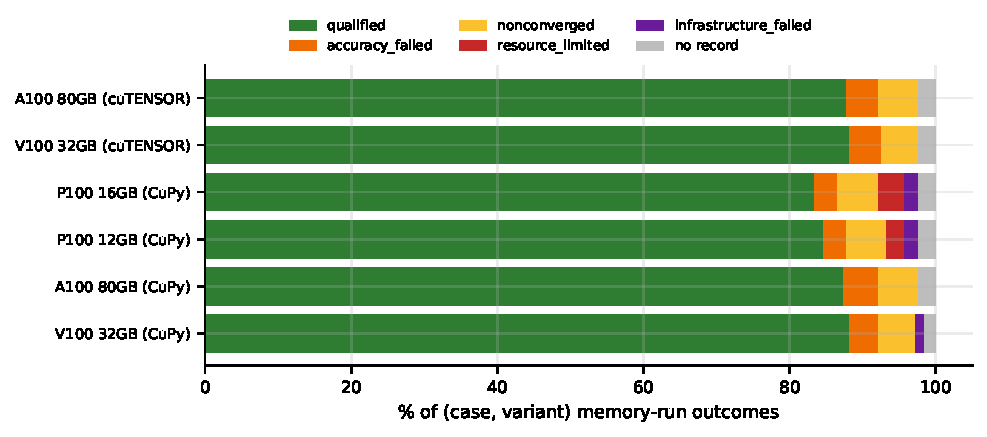
\includegraphics[width=.82\textwidth]{fig_status.pdf}
\caption{Outcome of the memory-mode run of each case and code version on each stratum. ``No record'' are the three open-shell cases (OH with B3LYP, PBE and wB97X) whose CPU reference did not converge and that were not run on the GPU, and the pre-launch rejections noted in Section~\ref{sec:limits}.}
\label{fig:status}
\end{figure}

\section{Accuracy}
\label{sec:accuracy}

\paragraph{Qualified results.} Among all qualified GPU results the largest deviation from CPU PySCF, for both code versions, was $8.6\times10^{-9}$~Eh in the SCF energy (the gate is $10^{-8}$), $9.0\times10^{-7}$~Eh/Bohr in a gradient component (gate $10^{-6}$), $9.6\times10^{-7}$~Eh/Bohr$^2$ in a Hessian element (gate $10^{-5}$), $2.1\times10^{-8}$~Eh in an excitation energy (gate $10^{-6}$), $2.8\times10^{-9}$~Eh in a correlation energy, $2.3\times10^{-7}$~a.u.\ in a polarizability component (gate $10^{-5}$) and $5.3\times10^{-5}$~ppm in a shielding. Figure~\ref{fig:accuracy} shows the distribution. The new code is not less accurate than the original: its worst qualified gradient error ($8.5\times10^{-8}$~Eh/Bohr, for NO with B3LYP on the P100-16) is an order of magnitude below the original's worst ($9.0\times10^{-7}$, tamoxifen B3LYP/def2-TZVP on the V100 with the CuPy engine), and over the 1314 pairs of error values compared the new code's error is smaller in 606, larger in 466 and equal in 242 (median ratio 1.00), so the two versions cannot be distinguished in accuracy at this level; their differences are far below the gates. The worst values lie close to the gates (the gates were set from the numerical noise of the independent CPU reference), so the check demonstrates agreement at the gate level and does not establish a tighter bound.

\begin{figure}[!htbp]
\centering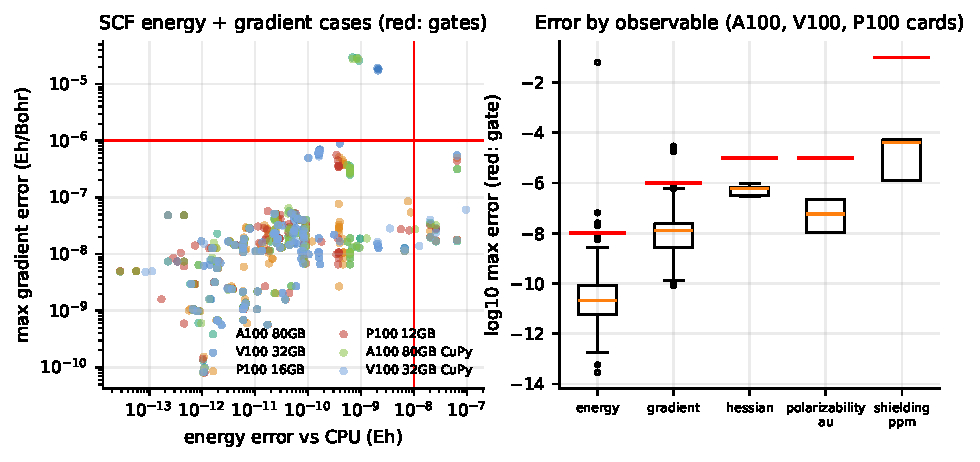
\includegraphics[width=\textwidth]{fig_accuracy.pdf}
\caption{Accuracy against the independent CPU result. Left: SCF energy and maximum gradient error of every energy-plus-gradient case that was run, for both code versions and all strata (red lines: gates; points beyond them are the failures listed in Table~\ref{tab:failures}). Right: log of the maximum error per observable over qualified results (red: gate).}
\label{fig:accuracy}
\end{figure}

\paragraph{Failures.} Table~\ref{tab:failures} lists every group of results that did not qualify. Two of them affect \emph{both} code versions identically on every card, so they are not caused by the changes under test, but are properties of the shared native stack, of the GPU methods or of a setup difference between the codes (not investigated): wB97M-V with its non-local correlation reproduces the CPU energy only to $2$--$6\times10^{-8}$~Eh for benzene, vitamin C and tamoxifen (it passes for H$_2$O at $6.6\times10^{-9}$), and the periodic MgO case differs by $6.4\times10^{-2}$~Eh while periodic silicon agrees to $5\times10^{-10}$~Eh. The wB97M-V offset grows with system size and is identical for the original and new code to the precision recorded; its cause was not investigated here.

\begin{table}[!htbp]
\centering\small
\begin{tabular}{p{4.6cm}p{2.2cm}p{6.7cm}}
\toprule
group & affects & observation \\
\midrule
Taxol HF, B3LYP, wB97X gradients & original only & maximum gradient error about $2\times10^{-5}$~Eh/Bohr against the gate $10^{-6}$; the new code passes (about $5\times10^{-9}$). No equal-accuracy ratio exists for these cases. \\
wB97M-V (benzene, vitamin C, tamoxifen) & both & energy error $2.6\times10^{-8}$, $2.0\times10^{-8}$, $6.4\times10^{-8}$~Eh (gate $10^{-8}$); gradients within the gate. \\
periodic MgO, $\Gamma$ point & both & energy differs by $6.4\times10^{-2}$~Eh on every card. \\
OH (B3LYP, PBE), NO (PBE), OH wB97X probe & all & CPU reference did not converge in 100 cycles from the MINAO guess; excluded. \\
benzene TDA and TDDFT & both & two of five roots flagged non-converged by the GPU solver at the declared tolerance; excitation energies agree with CPU to $1.2\times10^{-9}$~Eh (diagnostic). \\
NO, B3LYP, 48-thread CPU repetitions & CPU lane & two of three repetitions differ from the 24-thread reference by $1.1$ and $1.3\times10^{-8}$~Eh; an ill-conditioned case. \\
CCSD on Pascal (P100) & both & native kernel launch error \texttt{fill\_int4c2e}; cause not diagnosed. \\
Taxol and tamoxifen/TZVP hybrids on P100 & both & GPU memory exhausted (Section~\ref{sec:memory}). \\
\bottomrule
\end{tabular}
\caption{Groups of results that did not qualify. ``Both'' means the original and the new code behave identically.}
\label{tab:failures}
\end{table}

\section{Speed on the datacenter GPUs with cuTENSOR}
\label{sec:speed}

With cuTENSOR installed (the default on the V100 and A100), the new code is \emph{not faster} than the original. Over the 110 cases for which both versions qualified, the median ratio of original to new time is \MedianAllAHund{} on the A100 (range \MinAllAHund--\MaxAllAHund) and \MedianAllVHund{} on the V100 (range \MinAllVHund--\MaxAllVHund); restricting to the \NBigAHund{} (A100) and \NBigVHund{} (V100) cases where the new code takes at least five seconds, so that start-up costs matter less, gives medians of \MedianBigAHund{} and \MedianBigVHund{} (Figure~\ref{fig:violin}). Every job family is within $\pm3\%$ of unity on both cards (Table~\ref{tab:families}): SCF geometric mean 1.00, Hessians 1.00--1.01, TDA/TDDFT 1.00, DF-MP2 and CCSD 0.97--1.01, properties 1.00--1.01, geometry optimizations 1.00--1.01, solvated calculations 0.99--1.00.

\begin{table*}[!htbp]
\centering
\small
\resizebox{\textwidth}{!}{%
\begin{tabular}{lrrrrrrr}
\toprule
family & cases & A100 & V100 & A100 CuPy & V100 CuPy & P100-16 & P100-12 \\
\midrule
correlation & 8 & 0.97 (8) & 1.00 (8) & 1.01 (8) & 1.01 (8) & 1.02 (6) & 0.96 (6) \\
hessian & 8 & 1.00 (8) & 1.01 (8) & 1.03 (8) & 1.02 (8) & 1.02 (8) & 1.02 (8) \\
optimization & 4 & 1.00 (4) & 1.01 (4) & 1.02 (4) & 1.02 (4) & 1.01 (4) & 1.03 (4) \\
pbc & 4 & 0.99 (3) & 1.02 (3) & 1.02 (3) & 1.02 (3) & 1.02 (3) & 1.01 (3) \\
properties & 6 & 1.00 (6) & 1.01 (6) & 1.00 (6) & 1.00 (6) & 1.00 (6) & 0.99 (6) \\
scf & 77 & 1.00 (67) & 1.00 (67) & 1.07 (66) & 1.05 (67) & 1.06 (63) & 1.09 (66) \\
solvent & 8 & 0.99 (8) & 1.00 (8) & 1.05 (8) & 1.05 (8) & 1.07 (8) & 1.14 (8) \\
td & 12 & 1.00 (6) & 1.00 (6) & 1.01 (6) & 1.01 (6) & 1.02 (6) & 1.02 (6) \\
\bottomrule
\end{tabular}}
\caption{Geometric mean of the time ratio original/new per job family (number of cases in brackets); only cases where both versions passed the accuracy gate are included. Values above 1 mean the new code is faster.}
\label{tab:families}
\end{table*}


\begin{figure}[!htbp]
\centering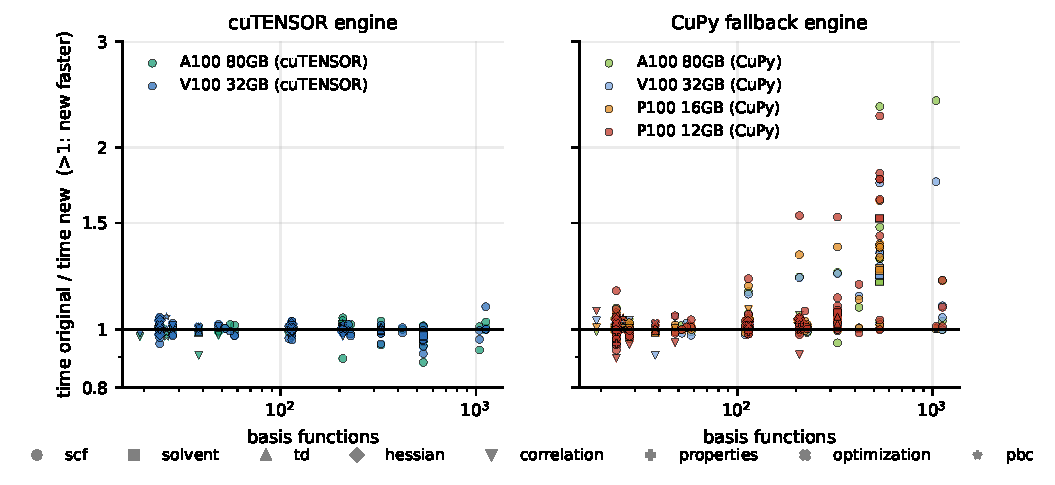
\includegraphics[width=\textwidth]{fig_speed_ratio_vs_size.pdf}
\caption{Time of the original code divided by time of the new code for every case in which both versions qualified, against the number of basis functions (marker shape = job family). Left: cuTENSOR engine. Right: CuPy fallback engine.}
\label{fig:ratio}
\end{figure}

\begin{figure}[!htbp]
\centering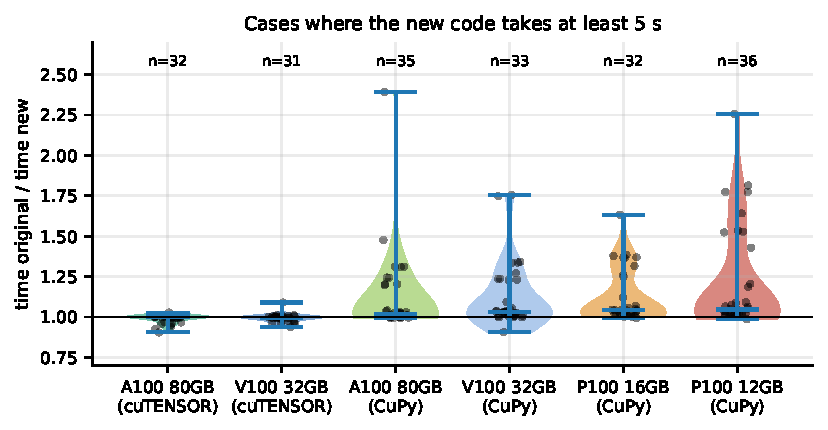
\includegraphics[width=.8\textwidth]{fig_speed_violin.pdf}
\caption{Distribution of the original/new time ratio over cases where the new code takes at least five seconds, per stratum (dots: individual cases).}
\label{fig:violin}
\end{figure}

The larger cases (Table~\ref{tab:large_cutensor}) show where the small differences occur. With the pure functionals LDA, PBE and TPSS the ratios are 0.99--1.09 (Taxol PBE: 1.03 on the A100 and 1.09 on the V100). For hybrid functionals the new code is slightly \emph{slower}: Hartree--Fock tamoxifen 0.88 (A100) and 0.91 (V100) and vitamin C 0.90 (A100), tamoxifen/B3LYP 0.96, tamoxifen/wB97X 0.94, tamoxifen/B3LYP in the larger def2-TZVP basis 0.92 (A100) and 0.96 (V100), and the PCM and SMD solvation cases 0.97. These differences of 3--12\% are small. They recur on both cards, which were measured on shared nodes and are not independent replicates, and they are consistent with the larger gradient cost of the memory-saving gradient (Section~\ref{sec:profile}), although the stage profile does not separate this cost from the other changes.

\begin{table}[!htbp]
\centering
\small
\begin{tabular}{lrrr}
\toprule
case & AOs & A100 & V100 \\
\midrule
\texttt{vitamin\_c-b3lyp-svp} & 208 & 2.34 / 1.04 & 2.18 / 1.01 \\
\texttt{inosine-b3lyp-svp} & 326 & 3.69 / 1.01 & 3.98 / 0.99 \\
\texttt{tamoxifen-lda-svp} & 537 & 4.67 / 1.00 & 4.81 / 0.99 \\
\texttt{tamoxifen-pbe-svp} & 537 & 5.34 / 1.01 & 5.70 / 1.01 \\
\texttt{tamoxifen-tpss-svp} & 537 & 8.05 / 1.01 & 8.72 / 1.00 \\
\texttt{tamoxifen-b3lyp-svp} & 537 & 6.49 / 0.96 & 7.80 / 0.96 \\
\texttt{tamoxifen-wb97x-svp} & 537 & 8.86 / 0.94 & 10.8 / 0.94 \\
\texttt{tamoxifen-pbe-tzvp} & 1042 & 8.48 / 1.01 & 10.8 / 1.00 \\
\texttt{tamoxifen-b3lyp-tzvp} & 1042 & 12.8 / 0.92 & 18.2 / 0.96 \\
\texttt{taxol-lda-svp} & 1123 & 14.5 / 1.01 & 18.3 / 1.00 \\
\texttt{taxol-pbe-svp} & 1123 & 18.0 / 1.03 & 24.2 / 1.09 \\
\texttt{taxol-tpss-svp} & 1123 & 26.4 / 1.00 & 38.1 / 1.00 \\
\texttt{taxol-hf-svp} & 1123 & 25.3 / (G0 acc.) & 47.5 / (G0 acc.) \\
\texttt{taxol-b3lyp-svp} & 1123 & 33.2 / (G0 acc.) & 58.8 / (G0 acc.) \\
\texttt{taxol-wb97x-svp} & 1123 & 49.1 / (G0 acc.) & 85.1 / (G0 acc.) \\
\texttt{tamoxifen-b3lyp-iefpcm} & 537 & 8.57 / 0.97 & 10.4 / 0.97 \\
\texttt{tamoxifen-b3lyp-smd} & 537 & 8.52 / 0.97 & 10.4 / 0.98 \\
\texttt{tamoxifen-wb97mv} & 537 & -- & -- \\
\texttt{vitamin\_c-b3lyp-hessian} & 208 & 20.1 / 1.00 & 20.9 / 0.99 \\
\texttt{inosine-b3lyp-tddft} & 326 & 8.99 / 1.00 & 9.87 / 1.01 \\
\bottomrule
\end{tabular}
\caption{Larger cases, cuTENSOR engine: new-code time in seconds / ratio original-over-new. `mem.' = did not fit in GPU memory or was refused by the memory forecast; `nc' = reference or GPU solver did not converge; `(G0 acc.)' = the original code fails the CPU accuracy gate, so no equal-accuracy ratio exists.}
\label{tab:large_cutensor}
\end{table}


\section{Speed without cuTENSOR: the CuPy fallback and the P100 cards}
\label{sec:engine}

The picture changes when contractions run through the CuPy \texttt{einsum} fallback, which is the only engine on the P100 cards and was forced on the V100 and A100 for a complete second stratum. The new code's Fock-build and gradient contractions use cuBLAS GEMM, GEMV and SYRK directly on this path, whereas the original code calls \texttt{einsum} and pays its repacking and temporaries. Over all cases the median original/new ratio is then \MedianAllAHundCupy{} (A100), \MedianAllVHundCupy{} (V100), \MedianAllPSixteen{} (P100-16) and \MedianAllPTwelve{} (P100-12); over the cases where the new code takes at least five seconds it is \MedianBigAHundCupy{}, \MedianBigVHundCupy{}, \MedianBigPSixteen{} and \MedianBigPTwelve{}, and the SCF family geometric mean is 1.05--1.09 (Table~\ref{tab:families}). The gain is largest in hybrid-functional cases of intermediate size (Table~\ref{tab:large_cupy}): tamoxifen with B3LYP 1.31 (A100) to 1.77 (P100-12), with wB97X 1.27--1.64, with PCM or SMD 1.20--1.53, and tamoxifen/B3LYP in def2-TZVP \MaxAllAHundCupy{} on the A100 and 1.76 on the V100; the GGA functionals gain little (PBE 1.00--1.04), whereas the meta-GGA TPSS, which has no exchange build, gains 1.24--1.43 for tamoxifen and 1.05--1.21 for Taxol (not investigated). The largest ratio observed in any stratum is \MaxAllAHundCupy{} (A100, CuPy engine).

\begin{table}[!htbp]
\centering
\small
\resizebox{\textwidth}{!}{%
\begin{tabular}{lrrrrr}
\toprule
case & AOs & A100 CuPy & V100 CuPy & P100-16 & P100-12 \\
\midrule
\texttt{vitamin\_c-b3lyp-svp} & 208 & 2.27 / 1.03 & 2.30 / 1.02 & 3.21 / 1.02 & 3.49 / 1.03 \\
\texttt{inosine-b3lyp-svp} & 326 & 4.00 / 1.02 & 4.39 / 1.05 & 6.55 / 1.05 & 7.01 / 1.09 \\
\texttt{tamoxifen-lda-svp} & 537 & 4.70 / 1.01 & 4.75 / 1.00 & 7.28 / 1.00 & 7.61 / 1.00 \\
\texttt{tamoxifen-pbe-svp} & 537 & 5.43 / 1.03 & 5.71 / 1.02 & 8.75 / 1.02 & 9.46 / 1.04 \\
\texttt{tamoxifen-tpss-svp} & 537 & 9.04 / 1.24 & 9.00 / 1.24 & 13.7 / 1.36 & 14.2 / 1.43 \\
\texttt{tamoxifen-b3lyp-svp} & 537 & 6.67 / 1.31 & 8.64 / 1.34 & 12.0 / 1.39 & 13.4 / 1.77 \\
\texttt{tamoxifen-wb97x-svp} & 537 & 9.20 / 1.48 & 12.2 / 1.27 & 16.8 / 1.32 & 19.2 / 1.64 \\
\texttt{tamoxifen-pbe-tzvp} & 1042 & 8.55 / 1.00 & 10.9 / 1.00 & 17.7 / 1.01 & 20.4 / 1.01 \\
\texttt{tamoxifen-b3lyp-tzvp} & 1042 & 12.7 / 2.39 & 18.5 / 1.76 & -- & -- \\
\texttt{taxol-lda-svp} & 1123 & 14.6 / 1.00 & 18.5 / 1.00 & -- & 34.5 / 1.01 \\
\texttt{taxol-pbe-svp} & 1123 & 17.9 / 1.03 & 24.3 / 1.09 & -- & 46.1 / 1.09 \\
\texttt{taxol-tpss-svp} & 1123 & 27.6 / 1.20 & 39.3 / 1.05 & -- & 69.8 / 1.21 \\
\texttt{taxol-hf-svp} & 1123 & 24.6 / (G0 acc.) & -- & mem. & mem. \\
\texttt{taxol-b3lyp-svp} & 1123 & 32.8 / (G0 acc.) & -- & mem. & mem. \\
\texttt{taxol-wb97x-svp} & 1123 & 48.5 / (G0 acc.) & -- & mem. & mem. \\
\texttt{tamoxifen-b3lyp-iefpcm} & 537 & 8.83 / 1.20 & 11.4 / 1.23 & 16.1 / 1.26 & 18.0 / 1.52 \\
\texttt{tamoxifen-b3lyp-smd} & 537 & 8.69 / 1.20 & 11.2 / 1.23 & 16.0 / 1.25 & 18.0 / 1.53 \\
\texttt{tamoxifen-wb97mv} & 537 & -- & -- & -- & -- \\
\texttt{vitamin\_c-b3lyp-hessian} & 208 & 26.1 / 1.04 & 25.3 / 1.04 & 37.8 / 1.04 & 36.3 / 1.04 \\
\texttt{inosine-b3lyp-tddft} & 326 & 10.2 / 1.01 & 11.6 / 1.03 & 17.1 / 1.07 & 21.4 / 1.05 \\
\bottomrule
\end{tabular}}
\caption{Larger cases, CuPy fallback engine: new-code time in seconds / ratio original-over-new. `mem.' = did not fit in GPU memory or was refused by the memory forecast; `nc' = reference or GPU solver did not converge; `(G0 acc.)' = the original code fails the CPU accuracy gate, so no equal-accuracy ratio exists.}
\label{tab:large_cupy}
\end{table}


Figure~\ref{fig:engine} shows why. It comes from separate, instrumented profile runs with synchronized stage timers, whose absolute times are about 2\,s above those of the main matrix (Table~\ref{tab:large_cutensor}) and are comparable only with one another. In these runs, for tamoxifen with B3LYP the original code takes 8.3 s with cuTENSOR on the A100 and 10.4 s with the CuPy engine (7.9 and 14.3 s on the V100), while the new code takes 8.7 and 8.8 s on the A100 (8.3 and 9.2 s on the V100): the new code makes the fallback engine as fast as cuTENSOR, but with cuTENSOR installed its fast paths are bypassed and it gains nothing. Put differently, the changes remove a penalty that only the fallback engine pays. This is the regime of the earlier GB10 study (Appendix~\ref{sec:gb10}), where speed-ups of 1.47 (tamoxifen) and 1.95 (Taxol) were measured without cuTENSOR; the cluster data reproduce the direction and show that it depends on the engine, but with smaller factors (1.2--1.8 for tamoxifen hybrids); the GB10 tamoxifen factor (1.47) lies within this range, and its Taxol factor (1.95) is not an equal-accuracy comparison.

\begin{figure}[!htbp]
\centering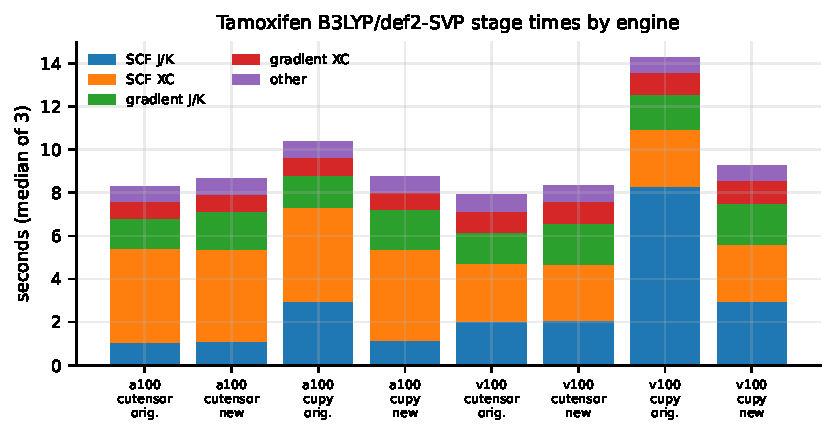
\includegraphics[width=.85\textwidth]{fig_engine_profile.pdf}
\caption{Stage times of tamoxifen B3LYP/def2-SVP (median of three, synchronized timers) for the original and new code with each engine. With cuTENSOR both versions take about 8--9 s; with the CuPy fallback the original code is slower (10.4 s on the A100, 14.3 s on the V100) and the new code is unchanged.}
\label{fig:engine}
\end{figure}

\section{Where the time goes and what did not help}
\label{sec:profile}

\paragraph{Stage profile.} Figure~\ref{fig:taxol} splits the Taxol B3LYP/def2-SVP workflow (20 SCF cycles) into stages. On the A100 the SCF takes 21.9 s (new code), of which the Fock build is 13.9 s (including 3.5 s to build the fitted integrals once), the XC quadrature 7.1 s and the diagonalization 0.4 s; the gradient takes 13.0 s, 76\% of it in the DF Coulomb and exchange derivatives. On the V100 the Fock build dominates even more (32.7 of 42.2 s SCF), as expected from its lower double-precision rate. The grid itself is built in about 0.1 s.

\begin{figure}[!htbp]
\centering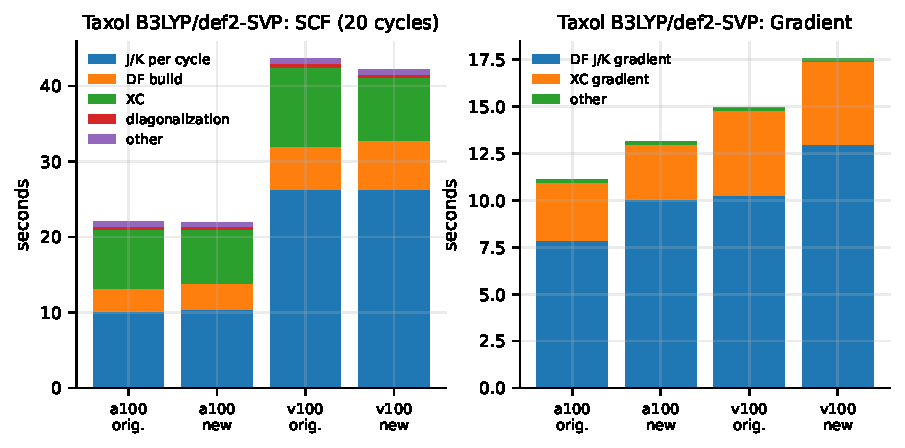
\includegraphics[width=\textwidth]{fig_taxol_stages.pdf}
\caption{Stage times of Taxol B3LYP/def2-SVP on the A100 and V100 with cuTENSOR, original (orig.) and new code. The new code's gradient is 2--3 s slower, the price of its much smaller gradient memory.}
\label{fig:taxol}
\end{figure}

\paragraph{The matrix products are near the measured cuBLAS rate.} A micro-benchmark of the exchange-build contractions at the real Taxol shapes (Figure~\ref{fig:gemm}) shows both the cuTENSOR path and the cuBLAS GEMM/SYRK path running at 14--15 TFLOPS on the A100 (the measured cuBLAS ceiling is 16.3) and 5.8 TFLOPS on the V100 (ceiling 6.8), i.e.\ 85--92\% of the measured cuBLAS rate for the best block sizes (a single block is timed and scaled to the full auxiliary basis, so these are not in-workflow rates); the GEMM/SYRK path is 0--13\% faster per cycle. There is little left to gain from tuning these products.

\begin{figure}[!htbp]
\centering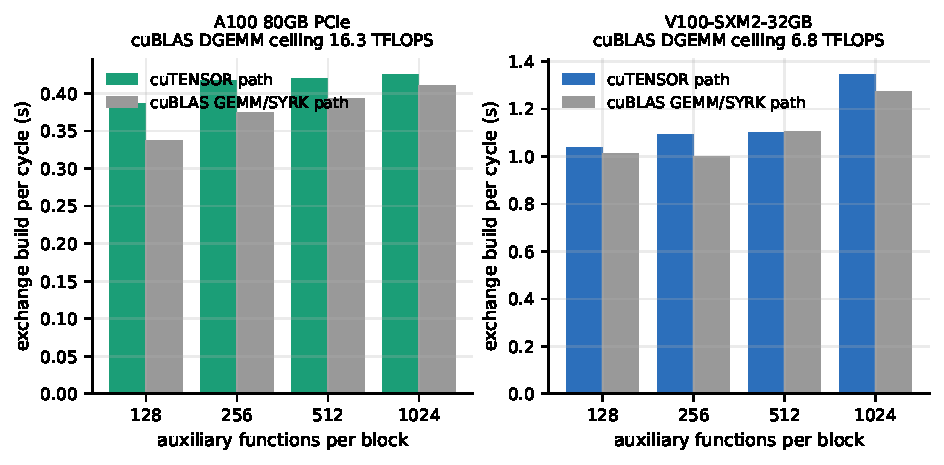
\includegraphics[width=.95\textwidth]{fig_gemm.pdf}
\caption{Estimated exchange-build time per SCF cycle for Taxol (one block of auxiliary functions timed, scaled to the full auxiliary basis) for the cuTENSOR contraction and the cuBLAS GEMM/SYRK path.}
\label{fig:gemm}
\end{figure}

\paragraph{Experiments that did not pay.}
\begin{itemize}[leftmargin=*,itemsep=1pt]
\item \emph{Gradient workspace cap.} Sweeping the fixed workspace budget of the new gradient (1, 2, 4, 8, 16\,GiB and unlimited) changed the Taxol gradient time by less than 1\% above 2\,GiB (13.0--13.1 s on the A100, 17.5--17.6 s on the V100), and by 8\% at 1\,GiB. The planner already chooses the same batch size at the default.
\item \emph{SCF cycle count.} Table~\ref{tab:cycles} and Figure~\ref{fig:cycles}: other starting guesses are equal (atomic densities) or much worse (H\"uckel, VSAP); a DIIS space of 12 saves one or two cycles; a two-stage scheme (coarse grid first) reduces the full-quality cycles from 20 to 12 for Taxol but its cheap pre-cycles cost as much (22.0 s against 22.2 s). Second-order SCF failed in all runs with a CuPy-to-NumPy conversion error.
\item \emph{Cached staging buffers for the disk tier} (a code-review suggestion): an alternating A/B/A/B comparison gave 265, 239~s (without) against 254, 280~s (with); the run-to-run spread exceeds any difference and the change was reverted.
\end{itemize}

\begin{table}[!htbp]
\centering
\small
\begin{tabular}{lrrr}
\toprule
strategy & vitamin C & tamoxifen & Taxol \\
\midrule
MINAO (baseline) & 18 / 3.8 & 18 / 6.0 & 20 / 22.2 \\
superposition of atomic densities & 18 / 4.0 & 19 / 6.0 & 21 / 22.5 \\
extended H\"uckel & 24 / 3.9 & 28 / 7.3 & 39 / 36.7 \\
superposition of atomic potentials & 23 / 5.7 & 27 / 24.7 & 39 / 153.2 \\
MINAO, DIIS space 12 & 16 / 3.5 & 17 / 5.7 & 19 / 21.6 \\
two-stage (coarse grid first) & 11 / 3.5 & 12 / 5.6 & 12 / 22.0 \\
second-order (SOSCF) & failed & failed & failed \\
\bottomrule
\end{tabular}
\caption{SCF cycles at full quality / total SCF seconds on the A100 for different starting guesses and convergence strategies (all reach the same energy within $10^{-8}$ Eh).}
\label{tab:cycles}
\end{table}

\begin{figure}[!htbp]
\centering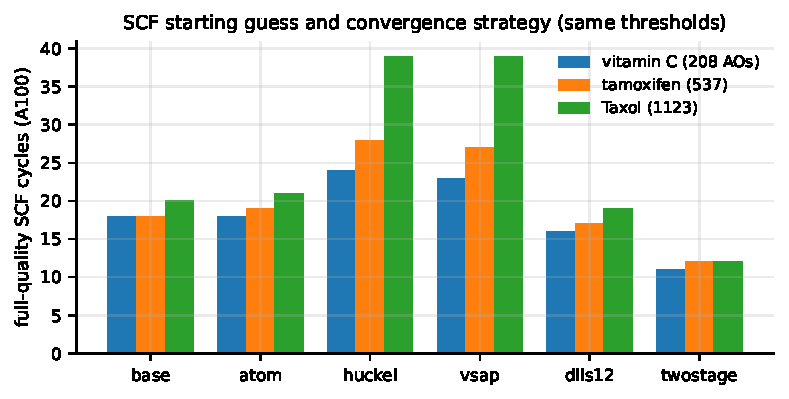
\includegraphics[width=.75\textwidth]{fig_scf_cycles.pdf}
\caption{SCF cycles at full quality for different starting guesses and convergence strategies on the A100.}
\label{fig:cycles}
\end{figure}

\section{First-process (cold start) cost}
\label{sec:cold}

CuPy compiles some kernels at run time. The first process on a node with an empty kernel cache therefore takes much longer than a repeat (Table~\ref{tab:cold} and Figure~\ref{fig:cold}): the H$_2$O B3LYP workflow takes 12.6--23.0 s the first time and 0.9--1.9 s with a populated cache, an overhead of 11--22 s that is similar for the original and the new code and is largest on the 12\,GB P100. The principal timings of this paper use a persistent cache; the figure matters mainly for short jobs and for users whose cache is not preserved between runs.

\begin{table}[!htbp]
\centering
\small
\resizebox{\textwidth}{!}{%
\begin{tabular}{lllrrrrr}
\toprule
card & engine & code & H$_2$O cold (s) & H$_2$O warm (s) & tamoxifen cold (s) & tamoxifen warm (s) & first-process overhead (s) \\
\midrule
A100 & cupy & original & 17.6 & 1.90 & 11.3 & 10.8 & 15.7 \\
 & cupy & new & 19.2 & 1.84 & 8.67 & 8.58 & 17.3 \\
 & cutensor & original & 19.6 & 1.94 & 8.36 & 8.14 & 17.7 \\
 & cutensor & new & 17.5 & 1.81 & 8.37 & 8.55 & 15.7 \\
V100 & cupy & original & 14.5 & 1.03 & 12.2 & 11.6 & 13.5 \\
 & cupy & new & 13.4 & 0.91 & 9.19 & 8.47 & 12.5 \\
 & cutensor & original & 13.0 & 0.86 & 7.56 & 7.37 & 12.2 \\
 & cutensor & new & 12.6 & 0.89 & 7.63 & 7.59 & 11.7 \\
P100-16 & cupy & original & 17.8 & 1.21 & 17.2 & 16.7 & 16.6 \\
 & cupy & new & 17.6 & 1.20 & 12.0 & 12.1 & 16.4 \\
P100-12 & cupy & original & 23.0 & 1.35 & 28.3 & 25.5 & 21.7 \\
 & cupy & new & 22.4 & 1.32 & 14.2 & 14.2 & 21.1 \\
\bottomrule
\end{tabular}}
\caption{Cold start: the first process with an empty CuPy kernel cache against a repeat with the cache populated (workflow time inside the process, imports excluded). Only the first process of each pass is truly cold, so the first-process overhead is the H$_2$O cold time minus its warm time; the later, larger cases of the cold pass reuse kernels compiled by H$_2$O.}
\label{tab:cold}
\end{table}

\begin{figure}[!htbp]
\centering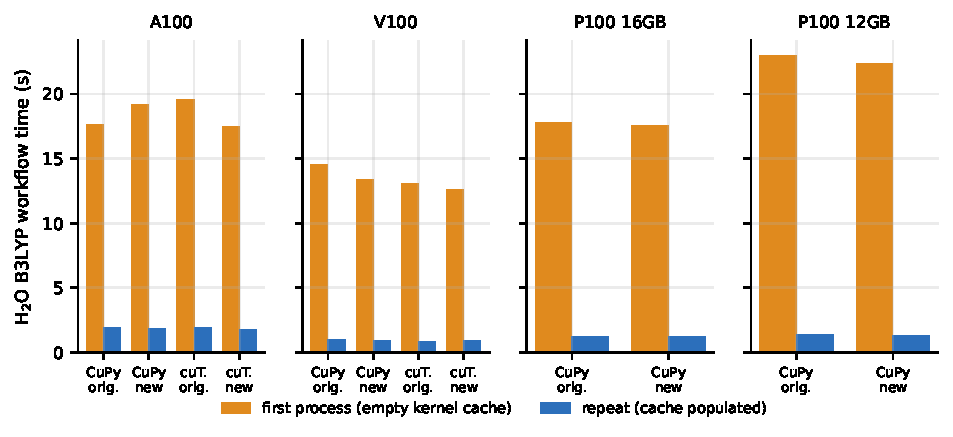
\includegraphics[width=\textwidth]{fig_cold_start.pdf}
\caption{H$_2$O B3LYP/def2-SVP workflow time in the first process after the kernel cache was emptied and in a repeat.}
\label{fig:cold}
\end{figure}

\section{CPU baseline and the GPU speed-up over the CPU}
\label{sec:cpu}

The study optimizes the GPU code, so the CPU is required only to be a fair baseline. The first CPU timing lane used a whole 48-core node with 48 OpenMP and BLAS threads, as the default whole-node setting. For mid-size systems this turned out to be a poor configuration: tamoxifen B3LYP/def2-SVP took 1663 s with 48 threads and default BLAS but 358 s with 24 threads in the scan (a single earlier 24-thread reference run, taken for the accuracy comparison and not as a timing measurement, took 519 s), with identical SCF iterations and energies. Over the complete 24-thread lane the same pattern holds: the 24-thread, one-BLAS-thread run was the faster lane in 120 of the 123 cases with both lanes; for the 65 cases that take at least 20\,s on 48 threads it is faster by a median of 2.0$\times$, and by up to 33$\times$ for the finite-difference benzene HF Hessian (4614 s against 141 s). A thread scan on the five representative cases (Table~\ref{tab:cpuscan}, Figure~\ref{fig:cpuscan}) found the cause: with 48 OpenMP threads each thread's BLAS calls spawn 48 more, oversubscribing the node. Setting BLAS threads to one restores the performance (tamoxifen 364 s at 48 threads, 307 s at 24 threads; vitamin C 24 s and 21 s against 55 s), pinning helps little, and for small molecules fewer threads are better still: benzene is fastest with 12 threads (4.0 s against 17.7 s with 48); H$_2$O is the exception, fastest with 48 threads (3.5 s), and for it and benzene the scan has no one-BLAS-thread runs. For Taxol with PBE the spread is 24\% (1594--1972 s). A second lane with 24 threads and one BLAS thread was therefore run for every case, and the fair CPU baseline of each case is the faster of the two lanes.

\begin{table*}[!htbp]
\centering
\small
\resizebox{\textwidth}{!}{%
\begin{tabular}{lrrrrrrrrrrr}
\toprule
case & 1 & 2 & 4 & 8 & 12 & 24 & 48 & 24/B1 & 48/B1 & 24 pin & 48 pin \\
\midrule
H$_2$O & 4.54 & 4.30 & 4.13 & 4.12 & 4.11 & 4.58 & \textbf{3.52} & -- & -- & -- & -- \\
benzene & 15.3 & 9.06 & 6.07 & 4.33 & \textbf{4.01} & 7.80 & 17.7 & -- & -- & -- & -- \\
vitamin C & -- & -- & -- & -- & 22.3 & 23.5 & 55.3 & \textbf{20.6} & 24.0 & 23.5 & 43.2 \\
tamoxifen & -- & -- & -- & -- & 319.8 & 357.8 & 1663 & \textbf{307.1} & 363.8 & 322.2 & 946.6 \\
Taxol PBE & -- & -- & -- & -- & 1972 & 1604 & 1717 & \textbf{1594} & 1622 & 1604 & 1700 \\
\bottomrule
\end{tabular}}
\caption{CPU thread scan, wall time in seconds on one 48-core node. Columns: OpenMP threads with BLAS threads equal to OpenMP threads; `B1' = BLAS threads set to 1; `pin' = OpenMP threads pinned to cores. Bold: fastest for that case.}
\label{tab:cpuscan}
\end{table*}

\begin{figure}[!htbp]
\centering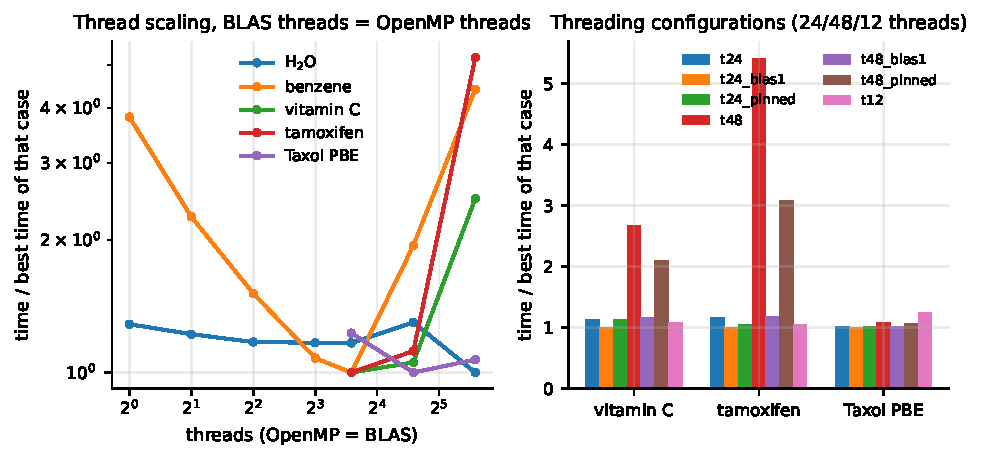
\includegraphics[width=\textwidth]{fig_cpu_scan.pdf}
\caption{CPU thread scaling. Left: time relative to the best configuration against thread count (BLAS threads equal to OpenMP threads). Right: threading configurations for the three larger cases.}
\label{fig:cpuscan}
\end{figure}

Table~\ref{tab:cpugpu} and Figure~\ref{fig:cpugpu} compare the CPU with the new GPU code. For the cases in which the CPU needs at least 20 s (\CPUNBestAHund{} on the A100, \CPUNBestVHund{} on the V100, \CPUNBestPSixteen{} on the P100-16) the median speed-up of the A100, V100 and P100-16 is \CPUMedBestAHund, \CPUMedBestVHund{} and \CPUMedBestPSixteen{} against the best CPU lane, with maxima of \CPUMaxBestAHund, \CPUMaxBestVHund{} and \CPUMaxBestPSixteen; the largest ratios belong to the finite-difference Hessians, which the CPU computes from many gradients. For small jobs the GPU gains little: it is slower than the best CPU lane in 39 of 113 cases on the A100 (36 and 38 on the V100 and P100-16) and less than three times faster in 56 A100 cases, among them (H$_2$O with HF, direct SCF, DF-MP2, CCSD, polarizability and shielding, and the formaldehyde wB97X TDA) with CPU times of a few seconds or less, where GPU start-up and small kernels dominate. The CPU baseline columns of the table state which lane was used.

\CPULaneNote

\begin{table*}[!htbp]
\centering
\small
\resizebox{\textwidth}{!}{%
\begin{tabular}{lrrrrrrr}
\toprule
case & AOs & CPU 48 thr (s) & CPU best (s) & A100 new (s) & V100 new (s) & P100-16 new (s) & speed-up A100 \\
\midrule
\texttt{h2o-b3lyp-svp} & 24 & 3.16 & 0.51 (cpu24b1) & 1.01 & 0.99 & 1.22 & 1 \\
\texttt{benzene-b3lyp-svp} & 114 & 17.7 & 3.67 (cpu24b1) & 1.28 & 1.31 & 1.69 & 3 \\
\texttt{vitamin\_c-b3lyp-svp} & 208 & 51.7 & 17.3 (cpu24b1) & 2.34 & 2.18 & 3.21 & 7 \\
\texttt{inosine-b3lyp-svp} & 326 & 118.8 & 72.4 (cpu24b1) & 3.69 & 3.98 & 6.55 & 20 \\
\texttt{tamoxifen-b3lyp-svp} & 537 & 1654 & 310.6 (cpu24b1) & 6.49 & 7.80 & 12.0 & 48 \\
\texttt{tamoxifen-b3lyp-tzvp} & 1042 & 683.0 & 593.6 (cpu24b1) & 12.8 & 18.2 & 26.0 & 46 \\
\texttt{taxol-pbe-svp} & 1123 & 1702 & 1604 (cpu24b1) & 18.0 & 24.2 & 39.3 & 89 \\
\texttt{taxol-tpss-svp} & 1123 & 2504 & 2063 (cpu24b1) & 26.4 & 38.1 & 60.6 & 78 \\
\texttt{vitamin\_c-b3lyp-hessian} & 208 & 20730 & 5268 (cpu24b1) & 20.1 & 20.9 & 37.8 & 262 \\
\texttt{inosine-b3lyp-tddft} & 326 & 949.1 & 790.2 (cpu24b1) & 8.99 & 9.87 & 17.1 & 88 \\
\texttt{tamoxifen-b3lyp-iefpcm} & 537 & 1931 & 927.4 (cpu24b1) & 8.57 & 10.4 & 16.1 & 108 \\
\texttt{vitamin\_c-dfmp2} & 208 & 18.7 & 2.13 (cpu24b1) & 1.11 & 1.17 & 1.59 & 2 \\
\bottomrule
\end{tabular}}
\caption{CPU wall time against the new GPU code. CPU 48 thr: whole 48-core node, default settings; CPU best: the faster of the available CPU lanes (configuration in brackets); speed-up = CPU best / A100.}
\label{tab:cpugpu}
\end{table*}

\begin{figure}[!htbp]
\centering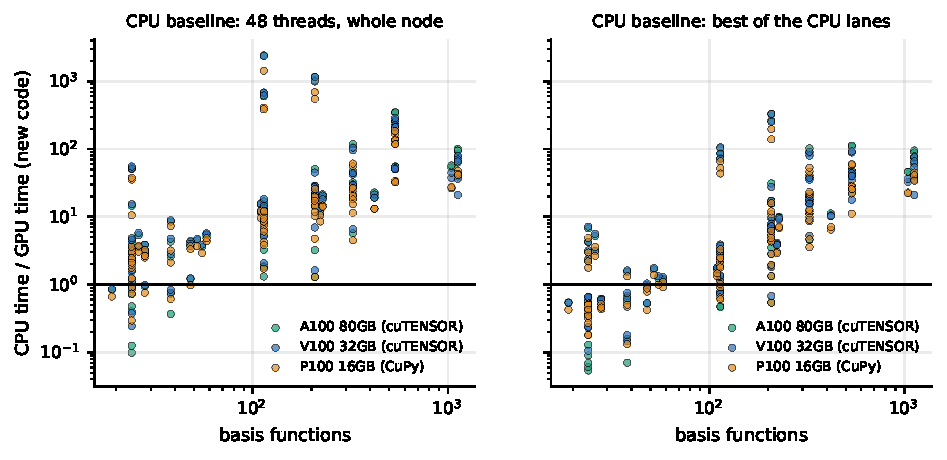
\includegraphics[width=\textwidth]{fig_cpu_vs_gpu.pdf}
\caption{CPU time divided by new-GPU time against system size. Left: CPU baseline from the 48-thread whole-node lane only. Right: baseline from the faster of the available CPU lanes.}
\label{fig:cpugpu}
\end{figure}

\section{Memory and capacity}
\label{sec:memory}

\subsection{GPU memory of the workflow}

The new code needs less GPU memory for every case that contains an exchange build and a gradient (Figure~\ref{fig:memory} and Table~\ref{tab:memory}). Over the \MemN{} cases with an original peak above 0.3~GB on the V100 the median reduction is \MemMedian$\times$ (range \MemMin--\MemMax$\times$): tamoxifen B3LYP falls from 15.9 to 4.4~GB (3.7$\times$), PCM and SMD cases 2.9--3.7$\times$, tamoxifen in def2-TZVP from 24.3 to 11.6~GB (2.1$\times$), and Taxol with the pure functionals LDA, PBE and TPSS 3.5--4.8$\times$ (from about 5 to 1--1.5~GB). Taxol with the hybrid functionals falls from 29.5 to 20.0~GB (HF, B3LYP; 1.5$\times$) and, for wB97X, from 29.6 to 25.9~GB (1.1$\times$). Hessians, TDA/TDDFT and DF-MP2 are unchanged (1.00$\times$): the changes do not touch their code paths, so the median above includes jobs that are not affected (over the 41 V100 cases with a reduction above 5\% it is 2.7$\times$). The figures depend on the stratum, because the original code sizes its gradient workspace from the free memory of the card: the medians are 1.8--2.5$\times$ over the six strata, the maxima 4.0--8.6$\times$, and the A100 maximum is Taxol with LDA (8.8 to 1.0~GB).

\begin{table}[!htbp]
\centering
\small
\begin{tabular}{lrrrr}
\toprule
case & AOs & original (GB) & new (GB) & ratio \\
\midrule
\texttt{vitamin\_c-b3lyp-svp} & 208 & 1.24 & 0.50 & 2.50 \\
\texttt{inosine-b3lyp-svp} & 326 & 4.60 & 1.29 & 3.58 \\
\texttt{tamoxifen-lda-svp} & 537 & 2.42 & 0.65 & 3.74 \\
\texttt{tamoxifen-b3lyp-svp} & 537 & 15.89 & 4.35 & 3.66 \\
\texttt{tamoxifen-wb97x-svp} & 537 & 15.93 & 5.20 & 3.07 \\
\texttt{tamoxifen-b3lyp-tzvp} & 1042 & 24.30 & 11.57 & 2.10 \\
\texttt{taxol-lda-svp} & 1123 & 4.89 & 1.02 & 4.78 \\
\texttt{taxol-pbe-svp} & 1123 & 5.06 & 1.42 & 3.56 \\
\texttt{taxol-tpss-svp} & 1123 & 5.08 & 1.45 & 3.51 \\
\texttt{taxol-hf-svp} & 1123 & 29.53 & 19.97 & 1.48 \\
\texttt{taxol-b3lyp-svp} & 1123 & 29.33 & 20.04 & 1.46 \\
\texttt{taxol-wb97x-svp} & 1123 & 29.57 & 25.85 & 1.14 \\
\texttt{tamoxifen-b3lyp-smd} & 537 & 16.51 & 4.47 & 3.69 \\
\texttt{vitamin\_c-b3lyp-hessian} & 208 & 2.57 & 2.57 & 1.00 \\
\texttt{inosine-b3lyp-tddft} & 326 & 5.58 & 5.58 & 1.00 \\
\texttt{vitamin\_c-dfmp2} & 208 & 0.80 & 0.80 & 1.00 \\
\bottomrule
\end{tabular}
\caption{Tracked GPU memory peak of the whole workflow on the V100 (memory-mode run; excludes the CuPy pool and native workspaces).}
\label{tab:memory}
\end{table}

\begin{figure}[!htbp]
\centering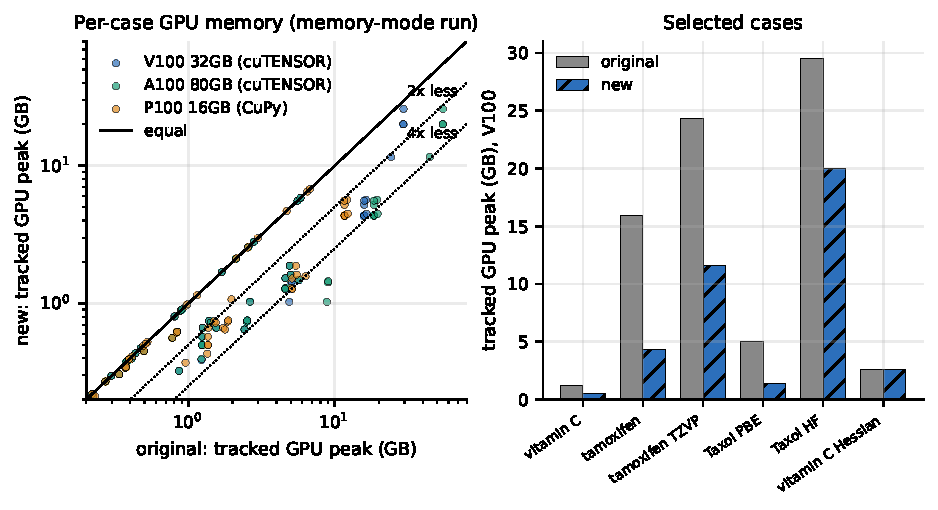
\includegraphics[width=\textwidth]{fig_memory.pdf}
\caption{Tracked GPU memory peak of the new against the original code. Left: every case with an original peak above 0.2~GB (the statistics in the text use 0.3~GB) on three strata (diagonal: equal; dotted: 2$\times$ and 4$\times$ less). Right: selected cases on the V100.}
\label{fig:memory}
\end{figure}

\subsection{Storage tiers}

The fitted integrals can be kept on the GPU, in pinned host memory, or (new code only) in a file read back in bounded blocks. Table~\ref{tab:storage} and Figure~\ref{fig:storage} give time and GPU memory for Taxol (which has a CPU reference and passes the accuracy gate in every tier for the new code) and for valinomycin (1542 basis functions, a capacity observation). Taxol on the V100 takes 59.3 s resident on the GPU, 71.7 s with the integrals in host memory (+21\%) and 254.5 s from disk, while the gradient-phase GPU peak falls to 4.1~GB in every tier (6.6~GB for the A100 disk run, which was made before the final gradient changes); the original code needs 29.6~GB for the gradient even with the integrals in host memory, and 54.9~GB on the A100. On the A100 the host tier costs +31\% (46.4 s against 35.4 s) because the faster card hides less of the transfer. On the 12 and 16~GB P100 cards neither the original code nor the GPU-resident new code can start Taxol with a hybrid functional (the 15.5~GB fitted-integral tensor alone does not fit), but the new code with host memory completes it in 111.5 and 91.5 s using 4.7~GB of GPU memory. Valinomycin does not fit the 32~GB V100 in either code version when resident (31.5~GB tensor); with host memory the original code needs 75.5~GB of GPU memory for its gradient (A100; this peak is card dependent, because the original workspace is sized from the free memory, and is not a minimum) while the new code needs 8.7~GB, so valinomycin runs on both P100 cards (265 s on the 12~GB and 221 s on the 16~GB card). The disk tier is 1.3--6$\times$ slower than host memory, depending on system and card (3--5.4$\times$ for Taxol and valinomycin); its times depend on the shared filesystem (Section~\ref{sec:limits}).

\begin{table}[!htbp]
\centering
\small
\resizebox{\textwidth}{!}{%
\begin{tabular}{lllrrr}
\toprule
system & card & version / tier & time (s) & GPU peak, gradient (GB) & host RSS (GB) \\
\midrule
Taxol (1123 AOs) & V100 32GB & orig. GPU & 59.1 & 29.6 & -- \\
 & V100 32GB & orig. host & 70.8 & 29.6 & 17 \\
 &  & new GPU & 59.3 & 4.1 & 1 \\
 &  & new host & 71.7 & 4.1 & 17 \\
 &  & new disk & 254.5 & 4.1 & 3 \\
 & A100 80GB & orig. GPU & 33.7 & 54.9 & -- \\
 & A100 80GB & orig. host & 43.8 & 54.9 & 17 \\
 &  & new GPU & 35.4 & 4.1 & 1 \\
 &  & new host & 46.4 & 4.1 & 17 \\
 &  & new disk & 215.2$^\dagger$ & 6.6$^\dagger$ & 3 \\
 & P100 16GB & orig. GPU & out of memory & -- & -- \\
 & P100 16GB & orig. host & out of memory & -- & -- \\
 &  & new host & 91.5 & 4.7 & 16 \\
 & P100 12GB & orig. GPU & out of memory & -- & -- \\
 & P100 12GB & orig. host & out of memory & -- & -- \\
 &  & new host & 111.5 & 4.7 & 16 \\
\midrule
valinomycin (1542 AOs) & V100 32GB & orig. GPU & out of memory & -- & -- \\
 & V100 32GB & orig. host & 174.4 & -- & 33 \\
 &  & new GPU & out of memory & -- & -- \\
 &  & new host & 185.0$^\dagger$ & 14.8$^\dagger$ & 33 \\
 &  & new disk & 577.6$^\dagger$ & 14.8$^\dagger$ & 6 \\
 & A100 80GB & orig. GPU & 79.4 & -- & 1 \\
 & A100 80GB & orig. host & 88.2 & 75.5 & 33 \\
 &  & new GPU & 79.1$^\dagger$ & 14.8$^\dagger$ & 1 \\
 &  & new host & 97.2 & 8.7 & 33 \\
 &  & new disk & 524.4$^\dagger$ & 14.8$^\dagger$ & 6 \\
 & P100 16GB & orig. host & out of memory & -- & -- \\
 &  & new host & 220.9 & 8.7 & 32 \\
 & P100 12GB & orig. host & out of memory & -- & -- \\
 &  & new host & 264.9 & 8.7 & 32 \\
\bottomrule
\end{tabular}}
\caption{Storage tiers for the fitted integrals. Taxol has a CPU reference and passes the accuracy gate for the new code in every tier (the original code fails its gradient gate); valinomycin is a capacity observation. The original code has no disk tier. Rows marked $\dagger$ were run before the final gradient-memory fixes (their gradient peaks are 6.6 and 14.8 GB instead of 4.1 and 8.7 GB); all other new-code rows use the final code.}
\label{tab:storage}
\end{table}

\begin{figure}[!htbp]
\centering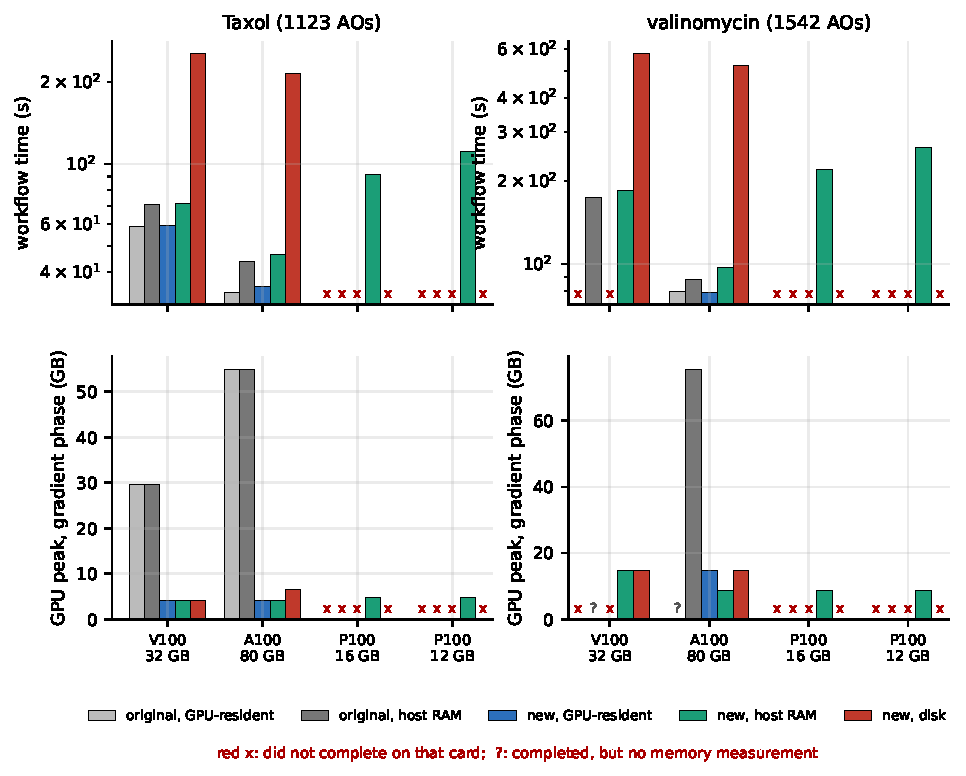
\includegraphics[width=\textwidth]{fig_storage_tiers.pdf}
\caption{Time (top) and gradient-phase GPU memory (bottom) of Taxol (left) and valinomycin (right) by storage tier and card.}
\label{fig:storage}
\end{figure}

\subsection{Capacity ladder}

Table~\ref{tab:capacity} and Figure~\ref{fig:capacity} give the largest system each code version and tier completed with a B3LYP/def2-SVP energy and full-response gradient. The new code completes a cluster of 139 water molecules (\BiggestAtoms{} atoms, \BiggestAOs{} basis functions) on the A100 in 17.9 min with host memory and 45.6 min from disk, against 300 atoms (2400 functions) for the original code; on the 32~GB V100 it reaches a 213-atom glycine chain (2154 functions) against a 76-water cluster of 228 atoms (1824 functions) for the original with host memory (the ladder mixes system families, and each entry is a lower bound at rung granularity), while resident on the GPU both versions stop at Taxol (1123 functions); on the two P100 cards it reaches valinomycin (168 atoms, 1542 functions) against tamoxifen (57 atoms, 537 functions) for the original, so a 12~GB card treats a system roughly three times larger (this P100 comparison mixes the memory and engine effects: the original code with host memory already reaches valinomycin on the 16~GB V100 with cuTENSOR); the 16~GB V100 reaches valinomycin with both versions (the original with host memory). These are capacity observations without a CPU reference.

\begin{table}[!htbp]
\centering
\small
\resizebox{\textwidth}{!}{%
\begin{tabular}{llcrrr}
\toprule
card & version / tier & largest system & atoms & AOs & time (min) \\
\midrule
P100 12GB & orig. GPU & tamoxifen & 57 & 537 & 0.39 \\
 & orig. host & tamoxifen & 57 & 537 & 0.42 \\
 & new GPU & tamoxifen & 57 & 537 & 0.22 \\
 & new host & valinomycin & 168 & 1542 & 4.41 \\
 & new disk & valinomycin & 168 & 1542 & 12.0 \\
\midrule
P100 16GB & orig. GPU & tamoxifen & 57 & 537 & 0.27 \\
 & orig. host & tamoxifen & 57 & 537 & 0.39 \\
 & new GPU & tamoxifen & 57 & 537 & 0.20 \\
 & new host & valinomycin & 168 & 1542 & 3.70 \\
 & new disk & valinomycin & 168 & 1542 & 12.9 \\
\midrule
V100 16GB & orig. GPU & tamoxifen & 57 & 537 & 0.13 \\
 & orig. host & valinomycin & 168 & 1542 & 3.17 \\
 & new GPU & tamoxifen & 57 & 537 & 0.14 \\
 & new host & valinomycin & 168 & 1542 & 3.05 \\
 & new disk & valinomycin & 168 & 1542 & 11.5 \\
\midrule
V100 32GB & orig. GPU & Taxol & 113 & 1123 & 0.94 \\
 & orig. host & (H$_2$O)$_{76}$ & 228 & 1824 & 4.54 \\
 & new GPU & Taxol & 113 & 1123 & 0.97 \\
 & new host & gly30 & 213 & 2154 & 8.99 \\
 & new disk & gly30 & 213 & 2154 & 11.7 \\
\midrule
A100 80GB & orig. GPU & (H$_2$O)$_{100}$ & 300 & 2400 & 4.29 \\
 & orig. host & (H$_2$O)$_{100}$ & 300 & 2400 & 4.58 \\
 & new GPU & gly40 & 283 & 2864 & 9.82 \\
 & new host & (H$_2$O)$_{139}$ & 417 & 3336 & 17.9 \\
 & new disk & (H$_2$O)$_{139}$ & 417 & 3336 & 45.6 \\
\bottomrule
\end{tabular}}
\caption{Largest system completed with B3LYP/def2-SVP energy and full-response gradient. These are capacity observations: no CPU reference exists, so only finite values and convergence are checked.}
\label{tab:capacity}
\end{table}

\begin{figure}[!htbp]
\centering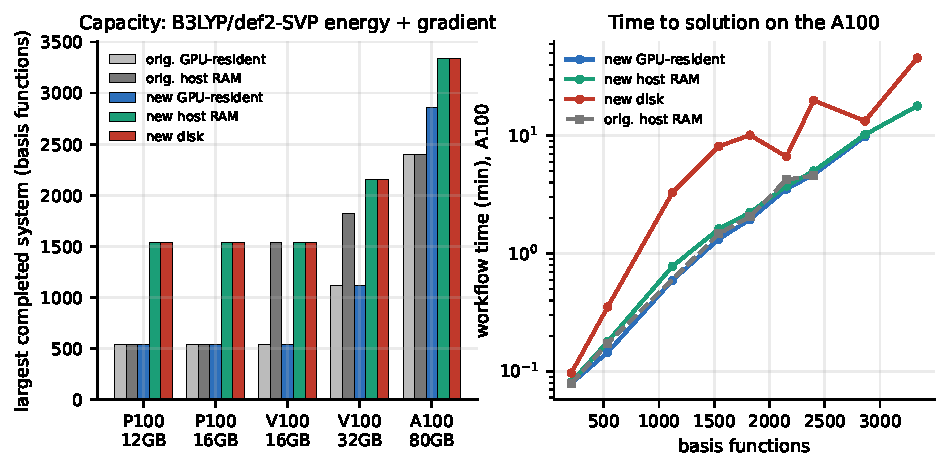
\includegraphics[width=\textwidth]{fig_capacity.pdf}
\caption{Left: largest system completed by card, code version and storage tier. Right: workflow time on the A100 against system size.}
\label{fig:capacity}
\end{figure}

\paragraph{What limits larger systems.} Beyond these rungs the limit is not the fitted-integral tensor but a tensor of $N_\mathrm{aux}N_\mathrm{occ}^2$ elements ($N_\mathrm{aux}$ counted in Cartesian functions) that the analytic gradient holds on the GPU whichever storage tier is used. It is 2.7~GB for Taxol, 6.4~GB for valinomycin, 26.6~GB for the 100-water cluster, 50.1~GB for the 40-residue glycine chain, 71.4~GB for the 139-water cluster, and 97.3~GB for the 50-residue chain, which exceeds the 80~GB of the A100 and ends the ladder there. The storage tiers of the fitted integrals are therefore exhausted at about 3300 basis functions on the largest card; going further requires the gradient to hold this tensor in host memory in blocks, which is not implemented.

\section{Discussion}
\label{sec:discussion}

\paragraph{What the changes buy.} (i) \emph{Memory}: a median of about 2$\times$ (1.8--2.5$\times$ by stratum) and up to 4.8$\times$ (V100) or 8.6$\times$ (A100) less tracked GPU memory, which together with the new disk tier and the host tier lets a 12~GB GPU treat systems of about 1500 basis functions and an 80~GB GPU systems of about 3300. (ii) \emph{Speed on the fallback engine}: 1.2--1.8$\times$ for intermediate-size hybrid-functional jobs, up to 2.4$\times$. (iii) \emph{No loss of accuracy}: the worst qualified errors are the same or smaller than for the original code. The changes do \emph{not} accelerate jobs that already use cuTENSOR, where the new code is on average 0--1\% different from the original and up to 12\% slower for Hartree--Fock and hybrid functionals in mid-size cases, nor jobs that do not call the modified paths directly (TDDFT, MP2, CCSD, properties, periodic; Hessians and optimizations differ by a few percent at most).

\paragraph{Relation to the earlier GB10 study.} The earlier study reported 1.47$\times$ for tamoxifen and 1.95$\times$ for Taxol (Table~\ref{tab:gb10}). Here the same direction appears only without cuTENSOR and with smaller factors; with cuTENSOR it disappears. The GB10 had no cuTENSOR bindings, much lower double-precision throughput and unified memory, so its result describes cards and installations without a working cuTENSOR (for example, hardware without cuTENSOR bindings) rather than datacenter GPUs.

\paragraph{Recommendations.} (1) Keep cuTENSOR as the default engine where available: over the cases where the new code takes at least five seconds, the CuPy engine makes the original code slower than cuTENSOR by a median of 1.12--1.14$\times$ and by up to 2.57$\times$ (tamoxifen B3LYP/def2-TZVP on the A100), while for the new code the median is 1.02--1.06$\times$ and the maximum 1.30$\times$ (this CuPy-over-cuTENSOR ratio is a different quantity from the original/new ratio quoted elsewhere). (2) Treat the new code's value on such systems as memory and capacity, and on fallback-engine systems also speed. (3) The next memory limit is the gradient tensor; offloading it to host memory in auxiliary blocks would extend all tiers. (4) The remaining time is dominated by the exchange build near the measured cuBLAS double-precision rate and, for mid-size systems, by the XC quadrature (73\% of the tamoxifen SCF on the A100), which is where further speed work would have to focus; neither start-up costs (Section~\ref{sec:cold}) nor the SCF cycle count offer large gains.

\section{Limitations and caveats}
\label{sec:limits}

\begin{itemize}[leftmargin=*,itemsep=2pt]
\item \textbf{Timing noise and sharing.} Timings come from fresh processes on shared cluster nodes. GPU nodes were not exclusive during the main matrix, so the other GPU of a two-GPU node (and the filesystem) may have been in use; medians over five to nine samples bound this (the spread of the individual cases is visible in Figures~\ref{fig:ratio} and~\ref{fig:violin}), but ratios within a few percent of one should be read as ``no difference''. Disk-tier timings depend on the page cache and the shared filesystem: two alternating runs of identical code on one node differed by up to 12\%, and repeated runs of Taxol on the V100 ranged from 239 to 280\,s. No general I/O performance claim is made; the disk-tier ratios refer to the specific runs and file system.
\item \textbf{Small systems.} Many core cases finish in one to a few seconds, where start-up costs, kernel launch latency and the CPU-side set-up dominate; ratios near one for these are expected and do not measure the numerical kernels.
\item \textbf{Memory figures} are the peak of requested live CuPy storage in a separate instrumented process. They exclude the CuPy pool overhead, cuTENSOR and cuBLAS workspaces and native allocations, so the real device footprint is somewhat higher, and the P100-16 rows that report \emph{resource limited} without a measurement are forecasts made by the scheduler before launch (they are labelled in the data).
\item \textbf{Capacity runs} have no independent reference; they are checked only for finite values and SCF convergence. The largest system with an accuracy-qualified comparison to CPU PySCF is Taxol.
\item \textbf{Registry amendments} (Section~\ref{sec:deviations}) change the numerical protocol relative to the original plan. In particular the GPU TDA calculations run at a tighter solver tolerance than the TDDFT calculations, so the TDA and TDDFT times must not be compared with each other; and the CPU Hessian timing is a finite-difference route, not PySCF's analytic Hessian.
\item \textbf{Non-converged and ill-conditioned cases.} Four open-shell cases do not converge on CPU and are excluded; two of the three 48-thread CPU repetitions of NO/B3LYP differ from the 24-thread reference by $1.1\times10^{-8}$ and $1.3\times10^{-8}$~Eh (gate $10^{-8}$) and are kept as accuracy failures; two of five benzene TDA and TDDFT roots are flagged non-converged by the GPU solver at the declared tolerance for both code versions, although the excitation energies agree with CPU to $1.2\times10^{-9}$~Eh.
\item \textbf{The original code fails the CPU gradient gate on Taxol} for HF, B3LYP and wB97X (maximum component error about $2\times10^{-5}$~Eh/Bohr), on all cards. Those cases have no equal-accuracy ratio.
\item \textbf{Runner labelling.} Plain CUDA out-of-memory errors (\texttt{cudaErrorMemoryAllocation}) are recorded by the runner as \emph{infrastructure failures}; they are genuine resource limits and are discussed as such. Pascal GPUs also fail CCSD with a native kernel launch error whose cause was not diagnosed.
\item \textbf{Audit tolerance.} The suite's audit demands exact equality of recomputed comparison statistics; last-digit differences between processes (multi-threaded reductions) required a wrapper that compares floating-point values to a relative $10^{-9}$ and everything else exactly. Pre-launch admission rejections are accepted without a request file only when they carry their forecast.
\item \textbf{Code-review findings left unchanged:} the 128\,MiB default staging buffer (the campaign sets it explicitly), the GGA density shortcut (empirically within every gate, but its sum-of-squares form is no longer exactly non-negative), the \texttt{strict\_grid\_order} compatibility flag, the missing early guard for disk tensors in the old DF-MP2 module, and a duplicated staging-cap check.
\item \textbf{CPU baseline.} The CPU is not optimized in this study. A 48-thread whole-node lane (the whole-node default) and a 24-thread, one-BLAS-thread lane are reported; the fair baseline for each case is the faster of the lanes. Other CPU settings (other thread counts, different BLAS) were not scanned for every case.
\end{itemize}

\section{Conclusions}
\label{sec:conclusions}

\begin{enumerate}[itemsep=2pt]
\item \textbf{The new GPU code is numerically equivalent to the original.} Across all qualified results, and across all job types and cards, the deviations from CPU PySCF are within the declared gates and not systematically different between the two code versions. The failures that remain are either the original code's own (Taxol gradients with hybrid functionals) or common to both versions, and so not caused by the changes under test (wB97M-V, periodic MgO; their cause was not investigated).
\item \textbf{Speed depends on the contraction engine.} With cuTENSOR the new code is no faster than the original (median ratio 1.00); without it, which is the case on the Pascal cards and on installations without a working cuTENSOR, it is faster by 1.2--1.8$\times$ for intermediate-size hybrid-functional calculations and by up to 2.4$\times$. The original code is the one that suffers from the loss of cuTENSOR.
\item \textbf{Memory is the main gain.} A median of about 2$\times$ (up to 4.8$\times$ on the V100 and 8.6$\times$ on the A100) less tracked GPU memory, plus a disk tier and a bounded build workspace, extend the reachable system size: valinomycin (1542 basis functions) on 12 and 16\,GB P100 cards, 3336 functions on the 80\,GB A100. The price of the host tier is 20--30\% of the run time and of the disk tier a factor of 1.3 to 6.
\item \textbf{The next limit is the gradient.} A tensor of size $N_\mathrm{aux}N_\mathrm{occ}^2$ (97\,GB for a 50-residue glycine chain) caps the system size on every card regardless of where the fitted integrals live; moving it to host memory in blocks is the most valuable next step.
\item \textbf{The exchange build is near the hardware ceiling.} The exchange matrix products run at 85--92\% of the measured cuBLAS double-precision rate; the SCF-cycle count, starting guess, gradient workspace budget and start-up cost offer little. Remaining speed work should target the XC quadrature, which is 73\% of the SCF time for tamoxifen on the A100 (32\% for Taxol).
\item \textbf{The CPU comparison must use a tuned baseline.} Using all 48 cores with default BLAS threading made CPU calculations slower than 24 threads with one BLAS thread in 120 of the 123 cases with both lanes (median 2.0$\times$ for the 65 cases above 20\,s on 48 threads; up to 33$\times$ for the benzene HF Hessian); GPU speed-ups over the CPU should be quoted against the better of the two.
\end{enumerate}


\section*{Data and code availability}
The code changes, the benchmark suite, the campaign drivers, the audited summary data and the sources of this manuscript are available at \url{https://github.com/qshao/gpu4pyscf} (branch \texttt{improve-single-gpu}). The frozen campaign is identified by the SHA-256 digest given in Appendix~\ref{sec:repro}. The raw per-job records (about 66\,GB) are not included in the repository and are available from the authors on request.

\appendix
\section{Reproducibility}
\label{sec:repro}

\paragraph{Frozen campaign.} The 127-case campaign (\texttt{campaign1}) was frozen on 2026-10-20 with the SHA-256 digest of its \texttt{campaign.json} \texttt{\scriptsize 231fea7a9e1722ad46b8c79eeb06789f0437118b8df3fa4976874d7459e4d380}. The file records the hashes of the G0 and G1 Python sources, the native libraries, all benchmark helper files, the registry and the hashed initial atomic densities; every job validates these identities before and after it runs, and each card works in a fork of the campaign whose \texttt{campaign.json} is byte-identical, so the CPU references are shared and one audit applies to all.

\paragraph{Layout.}
The code, benchmark suite and manuscript sources are in the \texttt{improve-single-gpu} branch of \url{https://github.com/qshao/gpu4pyscf} (commit \texttt{ac154f9} at submission). Code and data live in \texttt{benchmarks/single\_gpu/qm\_suite} of the repository (\texttt{cases.json}, \texttt{run.py}, \texttt{schedule.py}, \texttt{adapters.py}, \texttt{audit.py}); the cluster drivers are in \texttt{qm\_suite/lcc}; the stage profiles, storage-tier and capacity runs are in \texttt{benchmarks/single\_gpu/lcc\_profile\_results}; the manuscript is built from \texttt{reports/lcc\_benchmark} (\texttt{collect\_aux.py}, \texttt{make\_figures.py}, \texttt{make\_tables.py}, \texttt{report.tex}). The environment is a conda environment with Python~3.11, PySCF~2.14.0, CuPy~13.4.1, cuTENSOR~2.2.0 and the GCC~12 and CUDA~12.4 toolchains.

\paragraph{Commands.} CPU references: a Slurm job array over the case list calling \texttt{run.py ... --variant CPU --mode reference}. GPU matrix: \texttt{schedule.py --campaign all --cases <list> --repetitions 5} on each card fork. CPU timing: \texttt{run.py ... --variant CPU --mode timing} per case and repetition on whole nodes. Capacity ladder: \texttt{lcc/capacity.py CARD}. Cross-stratum tables: \texttt{lcc/compare\_variants.py}.

\section{Context: earlier single-GPU study on a GB10}
\label{sec:gb10}

Before the cluster campaign, the same branch was compared with the original code on one NVIDIA GB10 (unified memory, weak double-precision throughput, no cuTENSOR bindings so all contractions used the CuPy fallback). Table~\ref{tab:gb10} reproduces that result. The GB10 study motivated two checks in the present report: whether the speed-up survives when cuTENSOR is available (Section~\ref{sec:engine}), and whether the memory reduction matters on cards with far less memory (Section~\ref{sec:memory}).

\begin{table}[!htbp]
\centering
\small
\resizebox{\textwidth}{!}{%
\begin{tabular}{lrrrrrrr}
\toprule
system & atoms & AOs & original (s) & new (s) & ratio & orig. GB & new GB \\
\midrule
Vitamin C & 20 & 208 & 5.49 & 5.28 & 1.04 & 1.4 & 0.5 \\
Tamoxifen & 57 & 537 & 70.5 & 48.1 & 1.47 & 21.1 & 4.3 \\
Taxol & 113 & 1123 & 1103 & 566.0 & 1.95 & 65.6 & 30.1 \\
\bottomrule
\end{tabular}}
\caption{Earlier study on one NVIDIA GB10 (unified memory, CuPy fallback contractions, B3LYP/def2-SVP, three timing repetitions); shown for context. The original code fails the CPU gradient gate on Taxol, so that ratio is not an equal-accuracy speed-up.}
\label{tab:gb10}
\end{table}


\begin{landscape}
\section{Per-case results}
\scriptsize\setlength{\tabcolsep}{3pt}
\begin{longtable}{lrrrrrrrrrrr}
\caption{Per-case results. Columns A100 to P100-12: time ratio original/new (``nc'': a solver or reference did not converge; ``mem'': resource limit; ``acc'': the original code fails the accuracy gate; ``--'': not run or not qualified). G1: new-code time on the V100; mem: V100 GPU memory original/new in GB; CPU: best CPU time.}\label{tab:percase}\\
\toprule
case & AOs & A100 & V100 & A100c & V100c & P100-16 & P100-12 & G1 V100 (s) & mem (GB) & CPU (s) \\
\midrule
\endfirsthead
\toprule case & AOs & A100 & V100 & A100c & V100c & P100-16 & P100-12 & G1 V100 (s) & mem (GB) & CPU (s) \\ \midrule \endhead
\bottomrule \endfoot
\texttt{c-acetate-b3lyp-svp} & 110 & 0.99 & 1.01 & 1.01 & 1.00 & 1.00 & 1.03 & 1.28 & 0.1/0.1 & 2.18 \\
\texttt{c-acetate-pbe-svp} & 110 & 1.00 & 0.97 & 1.00 & 0.98 & 0.99 & 1.01 & 1.37 & 0.1/0.1 & 2.45 \\
\texttt{c-benzene-b3lyp-svp} & 114 & 0.99 & 0.98 & 1.01 & 1.01 & 1.00 & 0.99 & 1.31 & 0.2/0.2 & 3.67 \\
\texttt{c-benzene-b3lyp-tzvp} & 222 & 1.01 & 1.02 & 1.02 & 1.01 & 1.03 & 1.07 & 1.59 & 0.9/0.3 & 6.26 \\
\texttt{c-benzene-hf-svp} & 114 & 1.02 & 1.03 & 1.02 & 1.04 & 1.01 & 1.06 & 0.77 & 0.2/0.1 & 0.86 \\
\texttt{c-benzene-lda-svp} & 114 & 0.99 & 0.98 & 1.02 & 1.01 & 1.00 & 1.01 & 1.20 & 0.1/0.1 & 2.79 \\
\texttt{c-benzene-pbe-svp} & 114 & 1.02 & 0.99 & 1.04 & 1.06 & 1.00 & 1.00 & 1.29 & 0.1/0.1 & 3.80 \\
\texttt{c-benzene-pbe-tzvp} & 222 & 1.00 & 0.99 & 1.00 & 1.01 & 0.99 & 1.02 & 1.55 & 0.2/0.2 & 5.96 \\
\texttt{c-benzene-tpss-svp} & 114 & 1.00 & 1.01 & 1.15 & 1.14 & 1.18 & 1.21 & 1.61 & 0.1/0.1 & 4.74 \\
\texttt{c-benzene-wb97x-svp} & 114 & 1.00 & 0.96 & 1.06 & 0.99 & 1.00 & 1.02 & 1.74 & 0.2/0.2 & 4.00 \\
\texttt{c-benzene\_dimer-b3lyp-svp} & 228 & 0.98 & 0.98 & 0.99 & 1.01 & 1.01 & 1.01 & 2.08 & 1.5/0.7 & 19.9 \\
\texttt{c-benzene\_dimer-pbe-svp} & 228 & 1.02 & 0.97 & 1.01 & 0.99 & 1.02 & 1.00 & 1.96 & 0.5/0.4 & 18.1 \\
\texttt{c-distorted\_h2o-b3lyp-svp} & 24 & 0.98 & 1.00 & 1.02 & 1.00 & 1.01 & 1.00 & 1.03 & 0.0/0.0 & 0.51 \\
\texttt{c-h2o-b3lyp-pvdz} & 24 & 1.01 & 0.95 & 1.00 & 0.98 & 0.99 & 0.97 & 1.06 & 0.0/0.0 & 0.49 \\
\texttt{c-h2o-b3lyp-svp} & 24 & 1.01 & 1.04 & 1.01 & 1.00 & 0.98 & 1.04 & 0.99 & 0.0/0.0 & 0.51 \\
\texttt{c-h2o-hf-svp} & 24 & 1.04 & 1.04 & 1.03 & 1.01 & 0.99 & 1.01 & 0.71 & 0.0/0.0 & 0.38 \\
\texttt{c-h2o-lda-svp} & 24 & 1.01 & 1.03 & 0.98 & 0.95 & 1.00 & 1.05 & 1.00 & 0.0/0.0 & 0.56 \\
\texttt{c-h2o-pbe-pvdz} & 24 & 1.01 & 1.01 & 1.01 & 1.03 & 0.97 & 1.00 & 0.98 & 0.0/0.0 & 0.60 \\
\texttt{c-h2o-pbe-svp} & 24 & 1.00 & 1.03 & 0.99 & 1.01 & 1.00 & 1.08 & 0.97 & 0.0/0.0 & 0.59 \\
\texttt{c-h2o-tpss-svp} & 24 & 1.02 & 1.01 & 1.08 & 1.05 & 1.07 & 1.16 & 1.02 & 0.0/0.0 & 0.67 \\
\texttt{c-h2o-wb97x-svp} & 24 & 0.99 & 0.98 & 0.99 & 1.01 & 1.01 & 1.02 & 1.16 & 0.0/0.0 & 0.52 \\
\texttt{c-inosine-b3lyp-svp} & 326 & 1.01 & 0.99 & 1.02 & 1.05 & 1.05 & 1.09 & 3.98 & 4.6/1.3 & 72.4 \\
\texttt{c-inosine-hf-svp} & 326 & 0.94 & 0.95 & 0.95 & 1.03 & 1.06 & 1.13 & 2.00 & 4.6/1.3 & 17.3 \\
\texttt{c-inosine-lda-svp} & 326 & 1.01 & 0.99 & 1.01 & 1.00 & 1.00 & 1.00 & 3.11 & 0.8/0.6 & 48.5 \\
\texttt{c-inosine-pbe-svp} & 326 & 1.03 & 1.02 & 1.03 & 1.02 & 1.02 & 1.03 & 3.81 & 0.8/0.6 & 68.2 \\
\texttt{c-inosine-tpss-svp} & 326 & 1.00 & 1.00 & 1.24 & 1.24 & 1.37 & 1.53 & 5.22 & 0.8/0.6 & 106.8 \\
\texttt{c-inosine-wb97x-svp} & 326 & 0.99 & 0.98 & 0.99 & 1.02 & 1.04 & 1.08 & 4.97 & 4.6/1.5 & 77.3 \\
\texttt{c-methylammonium-b3lyp-svp} & 58 & 1.02 & 0.98 & 1.01 & 0.98 & 1.00 & 1.04 & 1.19 & 0.1/0.1 & 1.37 \\
\texttt{c-methylammonium-pbe-svp} & 58 & 0.99 & 0.98 & 0.99 & 1.01 & 1.01 & 1.01 & 1.22 & 0.1/0.1 & 1.57 \\
\texttt{c-no-b3lyp-svp} & 28 & 1.01 & 0.98 & acc & acc & 1.02 & 0.98 & 1.11 & 0.0/0.0 & 0.63 \\
\texttt{c-no-pbe-svp} & 28 & nc & nc & nc & 0.98 & -- & nc & 1.07 & 0.0/0.0 & -- \\
\texttt{c-o2-b3lyp-svp} & 28 & 0.98 & 1.01 & 1.00 & 1.00 & 1.01 & 0.97 & 1.01 & 0.0/0.0 & 0.56 \\
\texttt{c-o2-pbe-svp} & 28 & 1.01 & 1.02 & 1.02 & 0.99 & 1.00 & 0.97 & 1.01 & 0.0/0.0 & 0.63 \\
\texttt{c-oh-b3lyp-svp} & 19 & -- & -- & -- & nc & -- & -- & -- & -- & -- \\
\texttt{c-oh-pbe-svp} & 19 & -- & -- & -- & -- & nc & -- & -- & -- & -- \\
\texttt{c-stretched\_n2-b3lyp-svp} & 28 & 1.00 & 0.98 & 0.97 & 1.00 & 1.03 & 1.00 & 0.96 & 0.0/0.0 & 0.47 \\
\texttt{c-tamoxifen-b3lyp-svp} & 537 & 0.96 & 0.96 & 1.31 & 1.34 & 1.39 & 1.77 & 7.80 & 15.9/4.3 & 310.6 \\
\texttt{c-tamoxifen-b3lyp-tzvp} & 1042 & 0.92 & 0.96 & 2.39 & 1.76 & -- & -- & 18.2 & 24.3/11.6 & 593.6 \\
\texttt{c-tamoxifen-hf-svp} & 537 & 0.88 & 0.91 & 2.34 & 1.75 & 1.63 & 2.26 & 4.61 & 15.8/4.3 & 82.2 \\
\texttt{c-tamoxifen-lda-svp} & 537 & 1.00 & 0.99 & 1.01 & 1.00 & 1.00 & 1.00 & 4.81 & 2.4/0.6 & 201.4 \\
\texttt{c-tamoxifen-pbe-svp} & 537 & 1.01 & 1.01 & 1.03 & 1.02 & 1.02 & 1.04 & 5.70 & 2.5/0.7 & 251.4 \\
\texttt{c-tamoxifen-pbe-tzvp} & 1042 & 1.01 & 1.00 & 1.00 & 1.00 & 1.01 & 1.01 & 10.8 & 2.6/1.0 & 392.7 \\
\texttt{c-tamoxifen-tpss-svp} & 537 & 1.01 & 1.00 & 1.24 & 1.24 & 1.36 & 1.43 & 8.72 & 2.5/0.8 & 381.9 \\
\texttt{c-tamoxifen-wb97x-svp} & 537 & 0.94 & 0.94 & 1.48 & 1.27 & 1.32 & 1.64 & 10.8 & 15.9/5.2 & 371.2 \\
\texttt{c-taxol-b3lyp-svp} & 1123 & acc & acc & acc & -- & mem & mem & 58.8 & 29.3/20.0 & 2472 \\
\texttt{c-taxol-hf-svp} & 1123 & acc & acc & acc & -- & mem & mem & 47.5 & 29.5/20.0 & 998.5 \\
\texttt{c-taxol-lda-svp} & 1123 & 1.01 & 1.00 & 1.00 & 1.00 & -- & 1.01 & 18.3 & 4.9/1.0 & 1377 \\
\texttt{c-taxol-pbe-svp} & 1123 & 1.03 & 1.09 & 1.03 & 1.09 & -- & 1.09 & 24.2 & 5.1/1.4 & 1604 \\
\texttt{c-taxol-tpss-svp} & 1123 & 1.00 & 1.00 & 1.20 & 1.05 & -- & 1.21 & 38.1 & 5.1/1.4 & 2063 \\
\texttt{c-taxol-wb97x-svp} & 1123 & acc & acc & acc & -- & mem & mem & 85.1 & 29.6/25.9 & 3006 \\
\texttt{c-vitamin\_c-b3lyp-svp} & 208 & 1.04 & 1.01 & 1.03 & 1.02 & 1.02 & 1.03 & 2.18 & 1.2/0.5 & 17.3 \\
\texttt{c-vitamin\_c-b3lyp-tzvp} & 420 & 1.00 & 0.99 & 1.09 & 1.14 & 1.12 & 1.19 & 3.24 & 5.7/1.5 & 34.0 \\
\texttt{c-vitamin\_c-hf-svp} & 208 & 0.89 & 0.99 & 1.02 & 1.00 & 1.03 & 1.02 & 1.08 & 1.2/0.4 & 4.62 \\
\texttt{c-vitamin\_c-lda-svp} & 208 & 0.99 & 0.99 & 1.00 & 0.99 & 0.99 & 1.00 & 2.03 & 0.3/0.3 & 12.3 \\
\texttt{c-vitamin\_c-pbe-svp} & 208 & 1.03 & 1.01 & 1.01 & 1.00 & 1.03 & 0.98 & 2.33 & 0.4/0.3 & 16.8 \\
\texttt{c-vitamin\_c-pbe-tzvp} & 420 & 1.00 & 1.01 & 1.00 & 1.01 & 1.00 & 0.99 & 3.19 & 0.4/0.4 & 32.7 \\
\texttt{c-vitamin\_c-tpss-svp} & 208 & 1.00 & 0.99 & 1.22 & 1.22 & 1.33 & 1.54 & 3.14 & 0.4/0.3 & 20.9 \\
\texttt{c-vitamin\_c-wb97x-svp} & 208 & 1.01 & 1.01 & 1.02 & 1.00 & 1.02 & 1.02 & 2.66 & 1.2/0.6 & 19.4 \\
\texttt{c-water\_dimer-b3lyp-svp} & 48 & 0.99 & 1.01 & 1.00 & 1.01 & 0.99 & 0.99 & 1.12 & 0.1/0.1 & 1.05 \\
\texttt{c-water\_dimer-pbe-svp} & 48 & 1.00 & 1.02 & 1.00 & 0.99 & 1.02 & 1.05 & 1.16 & 0.1/0.1 & 1.21 \\
\texttt{direct-benzene-b3lyp} & 114 & 1.00 & 1.00 & 0.99 & 0.99 & 1.00 & 1.00 & 2.13 & 0.2/0.2 & 6.45 \\
\texttt{direct-benzene-hf} & 114 & 1.00 & 1.01 & 0.99 & 0.99 & 0.99 & 0.98 & 1.61 & 0.2/0.2 & 3.66 \\
\texttt{direct-benzene-pbe} & 114 & 1.00 & 1.03 & 1.00 & 0.98 & 0.99 & 1.02 & 1.62 & 0.2/0.2 & 6.30 \\
\texttt{direct-h2o-b3lyp} & 24 & 1.00 & 1.02 & 1.00 & 0.98 & 1.01 & 0.98 & 1.41 & 0.2/0.2 & 0.55 \\
\texttt{direct-h2o-hf} & 24 & 1.00 & 0.99 & 1.00 & 1.03 & 0.97 & 1.02 & 1.10 & 0.2/0.2 & 0.38 \\
\texttt{direct-h2o-pbe} & 24 & 0.99 & 1.05 & 0.98 & 1.01 & 1.01 & 1.01 & 0.97 & 0.2/0.2 & 0.50 \\
\texttt{e-benzene-b3lyp-hessian} & 114 & 1.00 & 1.00 & 1.04 & 1.03 & 1.04 & 1.02 & 8.07 & 0.4/0.4 & 699.3 \\
\texttt{e-benzene-b3lyp-tda} & 114 & nc & nc & nc & nc & nc & nc & -- & 0.4/0.4 & 66.7 \\
\texttt{e-benzene-b3lyp-tddft} & 114 & nc & nc & nc & nc & nc & nc & -- & 0.9/0.9 & 32.9 \\
\texttt{e-benzene-dfmp2} & 114 & 0.96 & 1.02 & 1.02 & 1.03 & 1.08 & 1.02 & 0.75 & 0.2/0.2 & 0.58 \\
\texttt{e-benzene-hf-hessian} & 114 & 1.01 & 1.02 & 1.04 & 1.01 & 1.04 & 1.01 & 1.95 & 0.3/0.3 & 140.7 \\
\texttt{e-benzene-optimization} & 114 & 1.00 & 1.01 & 1.02 & 1.05 & 1.02 & 1.01 & 5.15 & 0.2/0.2 & 19.2 \\
\texttt{e-benzene-pbe-hessian} & 114 & 1.00 & 1.01 & 1.02 & 1.03 & 1.04 & 1.03 & 7.71 & 0.5/0.5 & 816.1 \\
\texttt{e-benzene-polarizability} & 114 & 1.00 & 1.01 & 0.99 & 0.98 & 1.01 & 0.99 & 2.90 & 0.1/0.1 & 3.94 \\
\texttt{e-benzene-shielding} & 114 & 1.00 & 0.99 & 1.00 & 1.00 & 1.01 & 1.01 & 7.51 & 0.2/0.2 & 5.52 \\
\texttt{e-benzene-wb97mv} & 114 & acc & acc & acc & acc & acc & acc & -- & 0.2/0.2 & 55.6 \\
\texttt{e-benzene-wb97x-tda} & 114 & nc & nc & nc & nc & nc & nc & -- & 0.4/0.4 & 159.9 \\
\texttt{e-benzene-wb97x-tddft} & 114 & nc & nc & nc & nc & nc & nc & -- & 0.9/0.9 & 62.7 \\
\texttt{e-ch3i-pbe-ecp} & 55 & 1.02 & 0.99 & 1.01 & 1.02 & 1.01 & 1.01 & 1.80 & 0.1/0.1 & 2.38 \\
\texttt{e-formaldehyde-b3lyp-tda} & 38 & 1.01 & 1.01 & 1.00 & 1.00 & 1.01 & 0.99 & 2.91 & 0.1/0.1 & 1.83 \\
\texttt{e-formaldehyde-b3lyp-tddft} & 38 & 0.99 & 1.00 & 1.01 & 0.99 & 0.99 & 1.01 & 1.52 & 0.1/0.1 & 2.46 \\
\texttt{e-formaldehyde-ccsd} & 38 & 0.91 & 1.00 & 1.00 & 0.91 & mem & mem & 8.38 & 0.1/0.1 & 1.22 \\
\texttt{e-formaldehyde-optimization} & 38 & 1.00 & 1.01 & 1.01 & 1.02 & 1.00 & 1.02 & 4.23 & 0.1/0.1 & 3.18 \\
\texttt{e-formaldehyde-wb97x-tda} & 38 & 0.99 & 0.99 & 0.99 & 1.00 & 1.01 & 1.01 & 10.9 & 0.1/0.1 & 1.96 \\
\texttt{e-formaldehyde-wb97x-tddft} & 38 & nc & nc & nc & nc & nc & nc & -- & 0.1/0.1 & 2.74 \\
\texttt{e-h2o-b3lyp-d3bj} & 24 & 1.02 & 0.97 & 1.01 & 1.04 & 1.02 & 0.92 & 0.98 & 0.0/0.0 & 0.49 \\
\texttt{e-h2o-b3lyp-d4} & 24 & 0.98 & 1.00 & 0.99 & 0.98 & 1.01 & 0.96 & 1.00 & 0.0/0.0 & 0.54 \\
\texttt{e-h2o-b3lyp-hessian} & 24 & 1.00 & 0.98 & 1.04 & 1.02 & 0.99 & 1.00 & 2.24 & 0.1/0.1 & 9.57 \\
\texttt{e-h2o-b3lyp-iefpcm} & 24 & 1.00 & 1.00 & 1.00 & 0.97 & 1.00 & 1.03 & 1.25 & 0.0/0.0 & 0.79 \\
\texttt{e-h2o-b3lyp-smd} & 24 & 0.99 & 1.03 & 1.00 & 0.95 & 0.97 & 1.01 & 1.23 & 0.0/0.0 & 0.81 \\
\texttt{e-h2o-ccsd} & 24 & 1.00 & 1.00 & 1.01 & 1.01 & mem & mem & 6.95 & 0.1/0.1 & 0.73 \\
\texttt{e-h2o-dfmp2} & 24 & 0.98 & 1.01 & 1.01 & 1.04 & 1.01 & 0.90 & 0.64 & 0.0/0.0 & 0.34 \\
\texttt{e-h2o-hf-hessian} & 24 & 1.00 & 1.01 & 1.01 & 1.01 & 1.02 & 1.04 & 1.29 & 0.0/0.0 & 4.14 \\
\texttt{e-h2o-optimization} & 24 & 1.00 & 1.02 & 1.00 & 1.00 & 1.01 & 1.02 & 2.74 & 0.0/0.0 & 1.40 \\
\texttt{e-h2o-pbe-hessian} & 24 & 1.01 & 1.03 & 1.01 & 1.02 & 1.01 & 1.00 & 2.14 & 0.1/0.1 & 15.3 \\
\texttt{e-h2o-polarizability} & 24 & 1.00 & 1.01 & 1.01 & 0.99 & 0.99 & 0.95 & 1.65 & 0.1/0.1 & 0.39 \\
\texttt{e-h2o-shielding} & 24 & 1.00 & 1.01 & 1.00 & 1.02 & 1.01 & 0.99 & 1.74 & 0.1/0.1 & 0.41 \\
\texttt{e-h2o-wb97mv} & 24 & 1.00 & 1.00 & 1.03 & 1.05 & 1.06 & 0.94 & 1.56 & 0.0/0.0 & 3.69 \\
\texttt{e-i2-pbe-ecp} & 52 & 1.00 & 1.00 & 1.02 & 0.99 & 1.00 & 1.00 & 1.38 & 0.1/0.1 & 2.42 \\
\texttt{e-inosine-b3lyp-iefpcm} & 326 & 0.99 & 0.99 & 1.01 & 1.03 & 1.04 & 1.06 & 5.30 & 4.9/1.9 & 186.7 \\
\texttt{e-inosine-b3lyp-smd} & 326 & 1.00 & 0.99 & 1.01 & 1.03 & 1.04 & 1.07 & 5.26 & 5.0/1.6 & 199.2 \\
\texttt{e-inosine-b3lyp-tda} & 326 & 1.00 & 1.01 & 1.01 & 1.01 & 1.01 & 1.02 & 131.5 & 1.7/1.7 & 688.8 \\
\texttt{e-inosine-b3lyp-tddft} & 326 & 1.00 & 1.01 & 1.01 & 1.03 & 1.07 & 1.05 & 9.87 & 5.6/5.6 & 790.2 \\
\texttt{e-inosine-wb97x-tda} & 326 & nc & nc & nc & nc & nc & nc & -- & 2.1/2.1 & 889.1 \\
\texttt{e-inosine-wb97x-tddft} & 326 & 1.00 & 1.00 & 1.01 & 1.03 & 1.06 & 1.05 & 15.6 & 5.8/5.8 & 1421 \\
\texttt{e-no-dfump2} & 28 & 1.00 & 1.01 & 1.03 & 1.03 & 1.00 & 0.94 & 0.71 & 0.0/0.0 & 0.43 \\
\texttt{e-oh-dfump2} & 19 & 0.97 & 0.99 & 0.99 & 1.03 & 1.01 & 1.07 & 0.69 & 0.0/0.0 & 0.38 \\
\texttt{e-tamoxifen-b3lyp-d3bj} & 537 & 0.96 & 0.96 & 1.31 & 1.34 & 1.38 & 1.81 & 7.80 & 15.9/4.3 & 308.9 \\
\texttt{e-tamoxifen-b3lyp-d4} & 537 & 0.95 & 0.96 & 1.31 & 1.34 & 1.37 & 1.77 & 7.73 & 15.9/4.3 & 310.3 \\
\texttt{e-tamoxifen-b3lyp-iefpcm} & 537 & 0.97 & 0.97 & 1.20 & 1.23 & 1.26 & 1.52 & 10.4 & 16.4/5.7 & 927.4 \\
\texttt{e-tamoxifen-b3lyp-smd} & 537 & 0.97 & 0.98 & 1.20 & 1.23 & 1.25 & 1.53 & 10.4 & 16.5/4.5 & 954.7 \\
\texttt{e-tamoxifen-wb97mv} & 537 & acc & acc & acc & acc & acc & acc & -- & 15.9/5.6 & 2768 \\
\texttt{e-vitamin\_c-b3lyp-hessian} & 208 & 1.00 & 0.99 & 1.04 & 1.04 & 1.04 & 1.04 & 20.9 & 2.6/2.6 & 5268 \\
\texttt{e-vitamin\_c-b3lyp-iefpcm} & 208 & 1.02 & 1.00 & 1.02 & 1.01 & 1.02 & 1.02 & 2.91 & 1.4/0.7 & 46.2 \\
\texttt{e-vitamin\_c-b3lyp-smd} & 208 & 1.01 & 1.00 & 1.02 & 1.01 & 1.01 & 1.04 & 2.93 & 1.4/0.7 & 50.3 \\
\texttt{e-vitamin\_c-dfmp2} & 208 & 1.01 & 0.97 & 1.06 & 1.03 & 1.03 & 0.91 & 1.17 & 0.8/0.8 & 2.13 \\
\texttt{e-vitamin\_c-optimization} & 208 & 1.00 & 1.00 & 1.03 & 1.02 & 1.03 & 1.04 & 48.6 & 1.2/0.5 & 479.3 \\
\texttt{e-vitamin\_c-pbe-hessian} & 208 & 1.01 & 1.00 & 1.03 & 1.04 & 1.02 & 1.04 & 18.7 & 2.8/2.8 & 6185 \\
\texttt{e-vitamin\_c-polarizability} & 208 & 1.00 & 1.01 & 1.01 & 1.00 & 1.00 & 1.00 & 7.21 & 0.2/0.2 & 20.6 \\
\texttt{e-vitamin\_c-shielding} & 208 & 1.00 & 1.00 & 1.00 & 1.01 & 1.01 & 1.01 & 28.0 & 0.3/0.3 & 19.1 \\
\texttt{e-vitamin\_c-wb97mv} & 208 & acc & acc & acc & acc & acc & acc & -- & 1.3/0.7 & 239.3 \\
\texttt{e-water\_dimer-dfmp2} & 48 & 0.98 & 1.01 & 1.00 & 1.04 & 1.00 & 0.95 & 0.67 & 0.0/0.0 & 0.36 \\
\texttt{pbc-mgo-gamma} & 27 & acc & acc & acc & acc & acc & acc & -- & 0.0/0.0 & 3.57 \\
\texttt{pbc-si-gamma} & 26 & 0.97 & 1.00 & 1.00 & 1.02 & 1.01 & 1.00 & 0.94 & 0.0/0.0 & 2.92 \\
\texttt{pbc-si-k222} & 26 & 0.98 & 1.05 & 1.01 & 1.03 & 1.04 & 1.04 & 1.40 & 0.2/0.2 & 7.84 \\
\texttt{pbc-si-supercell-gamma} & 208 & 1.00 & 1.02 & 1.04 & 1.03 & 1.00 & 0.99 & 2.12 & 0.1/0.1 & 58.6 \\
\texttt{probe-oh-wb97x-svp} & 19 & -- & -- & -- & -- & -- & -- & -- & -- & -- \\
\end{longtable}

\end{landscape}


\begin{thebibliography}{99}\small
\bibitem{sun2018pyscf} Q.~Sun, T.~C.~Berkelbach, N.~S.~Blunt, G.~H.~Booth, S.~Guo, Z.~Li, J.~Liu, J.~D.~McClain, E.~R.~Sayfutyarova, S.~Sharma, S.~Wouters, G.~K.-L.~Chan, PySCF: the Python-based simulations of chemistry framework, \emph{WIREs Comput.\ Mol.\ Sci.}\ \textbf{8}, e1340 (2018).
\bibitem{sun2020pyscf} Q.~Sun, X.~Zhang, S.~Banerjee, P.~Bao, M.~Barbry, N.~S.~Blunt, \emph{et al.}, Recent developments in the PySCF program package, \emph{J.\ Chem.\ Phys.}\ \textbf{153}, 024109 (2020).
\bibitem{li2024gpu4pyscf} R.~Li, Q.~Sun, X.~Zhang, G.~K.-L.~Chan, Introducing GPU-acceleration into the Python-based Simulations of Chemistry Framework, arXiv:2407.09700 (2024).
\bibitem{wu2024gpu4pyscf} X.~Wu, Q.~Sun, Z.~Pu, T.~Zheng, W.~Ma, W.~Yan, X.~Yu, Z.~Wu, M.~Huo, X.~Li, W.~Ren, S.~Gong, Y.~Zhang, W.~Gao, Enhancing GPU-acceleration in the Python-based Simulations of Chemistry Framework, arXiv:2404.09452 (2024).
\bibitem{whitten1973} J.~L.~Whitten, Coulombic potential energy integrals and approximations, \emph{J.\ Chem.\ Phys.}\ \textbf{58}, 4496 (1973).
\bibitem{dunlap1979} B.~I.~Dunlap, J.~W.~D.~Connolly, J.~R.~Sabin, On some approximations in applications of $X\alpha$ theory, \emph{J.\ Chem.\ Phys.}\ \textbf{71}, 3396 (1979).
\bibitem{vahtras1993} O.~Vahtras, J.~Almlöf, M.~W.~Feyereisen, Integral approximations for LCAO-SCF calculations, \emph{Chem.\ Phys.\ Lett.}\ \textbf{213}, 514 (1993).
\bibitem{weigend2005} F.~Weigend, R.~Ahlrichs, Balanced basis sets of split valence, triple zeta valence and quadruple zeta valence quality for H to Rn, \emph{Phys.\ Chem.\ Chem.\ Phys.}\ \textbf{7}, 3297 (2005).
\bibitem{weigend2006} F.~Weigend, Accurate Coulomb-fitting basis sets for H to Rn, \emph{Phys.\ Chem.\ Chem.\ Phys.}\ \textbf{8}, 1057 (2006).
\bibitem{lehtola2018libxc} S.~Lehtola, C.~Steigemann, M.~J.~T.~Oliveira, M.~A.~L.~Marques, Recent developments in Libxc --- a comprehensive library of functionals for density functional theory, \emph{SoftwareX} \textbf{7}, 1 (2018).
\bibitem{okuta2017cupy} R.~Okuta, Y.~Unno, D.~Nishino, S.~Hido, C.~Loomis, CuPy: a NumPy-compatible library for NVIDIA GPU calculations, in \emph{Proc.\ Workshop on Machine Learning Systems (LearningSys) at NIPS} (2017).
\bibitem{cutensor} NVIDIA Corporation, cuTENSOR: a high-performance CUDA library for tensor primitives, \url{https://developer.nvidia.com/cutensor}.
\bibitem{mardirossian2016} N.~Mardirossian, M.~Head-Gordon, $\omega$B97M-V: a combinatorially optimized, range-separated hybrid, meta-GGA density functional with VV10 nonlocal correlation, \emph{J.\ Chem.\ Phys.}\ \textbf{144}, 214110 (2016).
\bibitem{grimme2011} S.~Grimme, S.~Ehrlich, L.~Goerigk, Effect of the damping function in dispersion corrected density functional theory, \emph{J.\ Comput.\ Chem.}\ \textbf{32}, 1456 (2011).
\bibitem{caldeweyher2019} E.~Caldeweyher, S.~Ehlert, A.~Hansen, H.~Neugebauer, S.~Spicher, C.~Bannwarth, S.~Grimme, A generally applicable atomic-charge dependent London dispersion correction, \emph{J.\ Chem.\ Phys.}\ \textbf{150}, 154122 (2019).
\end{thebibliography}

\end{document}
